\documentclass{article}
\usepackage{arxiv}  % 导入 arxiv 包
\usepackage[utf8]{inputenc}  % enable Unicode input
\usepackage[T1]{fontenc}
\usepackage{textcomp}        % extra text symbols (dash, quotes, etc.)
\usepackage{lmodern}         % vector fonts with extended glyph set
\usepackage{hyperref, url}   % 超链接
\usepackage{booktabs}  % 三线表
\usepackage{amsmath,amssymb,amsfonts}  % 数学支持
\usepackage{nicefrac}  % 优化行内分式排版
\usepackage{microtype}
\usepackage{multirow}  % 用于表格中跨行单元格
% \usepackage{lipsum}
\usepackage{graphicx, wrapfig}  % 图片插入, 多图并排
\usepackage{algorithm}  % 伪代码
\usepackage{algorithmic}
\newenvironment{proof}{{\noindent\it Proof}\quad}{\hfill $\square$\par}
\usepackage{listings}  % 插入代码
\usepackage{xcolor}  % 需要引入 xcolor 以支持颜色
\usepackage[font=small,labelfont=bf]{caption}

% Fix missing Unicode punctuation in ptmr8t
\DeclareUnicodeCharacter{2013}{--}   % en‐dash
\DeclareUnicodeCharacter{2014}{---}  % em‐dash
\DeclareUnicodeCharacter{2018}{`}    % left single quote
\DeclareUnicodeCharacter{2019}{'}    % right single quote
\DeclareUnicodeCharacter{201C}{``}   % left double quote
\DeclareUnicodeCharacter{201D}{''}   % right double quote
\bibliographystyle{IEEEtran}  % 参考文献格式
\date{This is a Technical Report, May 13\textsuperscript{th}, 2025}

\title{YOLO11-Earth: Training a Toy Remote Sensing Open Vocabulary Detector at only \$21}
\author{
    Zhicheng Xu \\
    School of Geographic Sciences, East China Normal University \\
    \texttt{zcxu@stu.ecnu.edu.cn}\\
}

\begin{document}
\maketitle

\begin{abstract}
Open Vocabulary Detection (OVD) aims to identify categories that the model has
never learnt before. Due to its cross-dataset transferability, it has become a
research hotspot. Existing OVD detectors consume a large amount of accelerator
memory during training and require multiple datasets from different tasks,
making the research threshold high. In the field of remote sensing images, the
object detection task faces problems such as large differences in dataset
category coverage and resolution, and a lack of detection models with strong
generalization ability. Open vocabulary detection is used to achieve
cross-dataset detection capabilities.

In response to this research status, this technical report introduces a lightweight
solution for open vocabulary detection in remote sensing images. This solution
fuses YOLOv11 and YOLOv8-Worldv2 and proposes a lightweight variant,
YOLOv11-Earth, through model pruning. It only uses the conventional xView
dataset and a consumer-grade GPU, enabling the traditional object detection
model YOLOv11 to have real-time open vocabulary detection capabilities on
remote sensing images. YOLOv11-Earth has been designed to optimize performance
while minimizing resource consumption, making it accessible for broader applications. 
In the DIOR zero-shot transfer test, YOLOv11-Earth outperforms the original
YOLOv8-Worldv2 and is comparable to its trained-on-xView version. In the DIOR
fine-tuning test, YOLOv11-Earth surpasses YOLOv8-Worldv2 and YOLOv11 when
using both partial and full fine-tuning training data, with an mAP50 of 84.5\%
for the x-sized model, demonstrating strong cross-dataset generalization
ability. YOLOv11-Earth can also transfer the pre-trained backbone network to
the YOLOv11-seg model and be applied to the in-box segmentation task on the
Potsdam dataset.

This study also uses machine learning theory to explain the source of
YOLOv11-Earth's open vocabulary detection ability. The lightweight design of
VL-PAN adds offline encoded text features as bias terms in the intermediate
process of the object detection model, achieving open vocabulary capabilities
but also resulting in the loss of zero-shot transferability.
\end{abstract}

\textbf{Keywords:} Open vocabulary detection, Remote sensing image processing, Model pruning, Transfer learning, Interpretability for AI

\section{Introduction}
Open Vocabulary Detection (OVD) has garnered significant attention in recent years, 
primarily due to its ability to identify objects or categories that a model has not 
encountered during its training phase \cite{zareian2021open, scheirer2012toward}. 
This capability is particularly crucial in the context of remote sensing imagery, 
where the diversity and complexity of objects necessitate models with robust 
generalization abilities. 

Traditional object detection models, such as RCNN, SSD, and YOLO, have shown remarkable 
performance in identifying objects within their training datasets \cite{girshick2014rich,liu2016ssd,redmon2016you}. 
However, these models often struggle when deployed in new environments with unseen 
categories, as they are inherently limited by the closed-set nature of their training \cite{akyon2022slicing,wu2022uiu,yang2022querydet}. 
To address this limitation, OVD models have been developed to extend the detection 
capabilities beyond the training dataset, enabling the identification of novel objects 
through the integration of additional modalities, such as textual information \cite{cheng2024yolo,liu2024grounding,ren2024grounding}. 

In this technical report, we aim to develop a lightweight OVD model tailored for remote sensing imagery. 
Our proposed model, YOLO11-Earth, integrates the strengths of YOLOv11 and YOLOv8-Worldv2 
while significantly reducing the computational requirements. 
This is achieved through model pruning and the use of a single, conventional dataset 
(xView) along with a consumer-grade GPU. 
The xView dataset, with its extensive coverage of various objects and high-resolution imagery, 
serves as the foundation for our pre-training process. 
By leveraging this dataset, we aim to equip YOLO11-Earth with the ability to perform 
real-time OVD on remote sensing images, thereby overcoming the limitations of existing 
models that require extensive computational resources and multiple datasets for training. 

The primary objectives of this research are threefold. 
Firstly, we focus on the design and pre-training of the lightweight OVD model, YOLO11-Earth, 
which involves reengineering the Vision-Language Path Aggregation Network (VL-PAN) to 
enhance multimodal prior learning. 
Secondly, we evaluate the cross-dataset and cross-task transfer learning capabilities 
of YOLO11-Earth through zero-shot transfer and fine-tuning experiments on the DIOR dataset, 
as well as by applying the model to the Potsdam segmentation dataset using YOLO11-seg. 
Lastly, we delve into the interpretability and potential improvements of YOLO11-Earth, 
comparing it with state-of-the-art models such as Grounding DINO and LAE-DINO to elucidate 
the sources of its OVD capabilities and identify areas for future enhancement. 

The remainder of this paper is organized as follows. 
Section 3 provides a detailed description of the datasets used for pre-training and evaluation, 
along with the data preprocessing methods. 
Section 4 outlines the experimental procedures and evaluation metrics, followed by a comprehensive 
presentation of the YOLO11-Earth model architecture and its differences from baseline models. 
Section 5 presents the experimental results, including pre-training performance, cross-dataset 
transfer learning outcomes, and cross-task transfer learning capabilities. 
Finally, Section 6 analyzes the low cost advantages and interpretability of YOLO11-Earth, and discusses potential improvements and future directions. 


\section{Related Work}

\subsection{Object Detection Models}
Existing object detection models can be categorized into 
two-stage detection models and one-stage detection models.  
Two-stage models, such as RCNN, Fast-RCNN, Faster-RCNN,  
and Mask-RCNN, first generate region proposals and then  
refine these proposals to detect and classify objects \cite{girshick2014rich,girshick2015fast,ren2016faster,he2017mask}.  
These models achieve high precision but require substantial  
computational resources and large datasets.  
In contrast, one-stage models like SSD and the YOLO series  
directly predict object locations and classes from the  
input image without generating region proposals.  
The YOLO series, in particular, has gained popularity due to  
its real-time detection capabilities on consumer-grade devices \cite{liu2016ssd,redmon2016you}.  
YOLOv2 (YOLO9000) and YOLOv3 introduced improvements in network  
structure and multi-scale feature handling \cite{redmon2017yolo9000,redmon2018yolov3}.  
YOLOv4 incorporated CIOU loss to enhance convergence speed  
and reduce bounding box confusion \cite{bochkovskiy2020yolov4}.  
YOLOv5 introduced multiple network sizes and was implemented  
entirely in PyTorch, making it easier to train and deploy \cite{jocher2020ultralytics}.  
YOLOv6 introduced anchor-free mechanisms and used EfficientRep  
and Rep-PAN for improved speed and performance \cite{li2022yolov6}.  
YOLOv7 adopted module-level reparameterization to optimize  
network parameters \cite{wang2023yolov7}.  
With the wide use of the Transformer architecture in computer Vision, object detectors based on 
ViT (Vision Transformer) have emerged. DETR is the first end-to-end object detection framework based 
on Transformer, avoiding non-end-to-end training and manually designed components in traditional detectors, 
such as non-maximum suppression (NMS), etc. \cite{carion2020end}. The proposal of DINO aims to further improve the performance 
of DETR-class models and introduces Contrastive De-noising Training. Technologies such as CDN, Mixed Query 
Selection and look forward twice \cite{zhang2022dino}. 
Its improvement works such as RT-DETR and Mask DINO have contributed in terms of performance \cite{li2023mask,zhao2024detrs,lv2024rt}.

At the same time, YOLOv8 further improved performance with better parameter  
utilization and faster training \cite{sohan2024review}.  
YOLOv9, v10, and 11 continued to enhance training strategies  
and receptive field sizes \cite{wang2024yolov9,wang2024yolov10,khanam2024yolov11}.  
YOLOv12 introduced attention mechanisms for improved dense  
object detection and classification \cite{tian2025yolov12}.  

\subsection{Open Vocabulary Detection Models}
Open Vocabulary Detection (OVD) models leverage multi-modal  
pre-training to align visual and textual features, enabling  
the detection of unseen categories.  
CLIP (Contrastive Language–Image Pretraining) has been a  
significant inspiration for OVD models, using contrastive  
learning to generate pseudo-labels and align text and  
image features \cite{radford2021learning}.  
Models like ViLD-text and ViLD-image have explored integrating  
language features into traditional object detection models  
like Mask-RCNN \cite{gu2021open}.  
GLIP further enhanced this approach by using a Swin-Transformer  
backbone and optimizing the balance between classification  
and localization losses \cite{li2022grounded,liu2021swin,zhang2022glipv2}.  
Grounding DINO combined the Transformer-based DINO detector  
with multi-modal pre-training, using composite datasets for  
language-image alignment \cite{liu2024grounding}.  
YOLO-World introduced a real-time OVD model by integrating  
CLIP’s text encoder and a reparameterizable visual-language  
path aggregation network (RepVL-PAN) \cite{cheng2024yolo}  
Subsequent models like YOLO-UniOW and YOLOE introduced adaptive  
decision learning and wildcard learning strategies to improve  
efficiency and adaptability \cite{liu2024yolo,sun2025yolo}.  
These models have demonstrated significant advancements in OVD,  
but they often require substantial computational resources for training.

\subsection{Remote Sensing Image Open Vocabulary Detection}
The application of OVD in remote sensing imagery has seen  
notable advancements with models like LAE-DINO, which introduced  
pseudo-label generation and text-image information filtering  
strategies \cite{pan2025locate}.  
LAE-DINO’s DVC module dynamically selects positive and negative  
vocabularies for each training batch, addressing the challenges  
of large-scale vocabulary sets.  
The VisGT module enhances text features by introducing “scene  
features,” which help align visual and textual features across  
the entire image.  
More recent models like OpenRSD have adopted multi-stage training  
processes—pre-training, fine-tuning, and self-training—to improve  
generalization capabilities \cite{huang2025openrsd}.  
These models have shown promise in enhancing the performance and  
efficiency of OVD in remote sensing imagery, but challenges remain  
in terms of computational costs and dataset requirements.

In summary, while significant progress has been made in both object  
detection and OVD, there is a need for lightweight models that can  
achieve real-time performance with reduced computational requirements.  
This study aims to address this gap by proposing a lightweight OVD  
model, YOLO11-Earth, designed specifically for remote sensing imagery.

\section{Benchmark Datasets and Preprocessing}

\subsection{Benchmark Dataset Selection}
The construction of the YOLO11-Earth model in this study 
follows the general paradigm of open vocabulary detection model construction:
first conducting pre-training on the xView dataset, which has the 
most labels and categories. Subsequently, zero-shot transfer, 
few-shot fine-tuning, and full fine-tuning experiments are carried 
out on the DIOR dataset, which has fewer labels and categories 
and lower difficulty. Finally, the YOLO11-seg model is initialized 
with the pre-trained YOLO11-Earth backbone network and fine-tuned 
on the Potsdam dataset for segmentation tasks. Unlike the majority 
of existing OVD research, YOLO11-Earth aims to achieve open vocabulary 
detection capabilities through pre-training on a closed training set.

The xView dataset \cite{lam2018xview} comprises images of complex scenes from around 
the world, annotated with bounding boxes and containing over a 
million object instances across 60 categories. The images have a 
spatial resolution of 0.3 m and cover an area exceeding 1,400 km² 
on the Earth's surface. The dataset includes various types of 
land cover and land use, except for China, and retains natural 
noise such as clouds and fog. The label and category distribution 
in xView is highly imbalanced, with significant variance in the 
area of bounding boxes within the same category. The purpose of 
pre-training on this dataset is to provide the model with as 
much prior knowledge as possible.

The DIOR dataset \cite{li2020object} contains 23,463 JPEG images and 190,288 instances, 
covering 20 target categories with spatial resolutions ranging 
from 0.5 m to 30 m. Similar to xView, the imaging conditions, 
weather, seasons, and image quality vary greatly, resulting in 
high inter-class similarity and intra-class diversity. This benchmark 
helps assess the cross-dataset transfer learning capabilities of 
YOLO11-Earth after pre-training. The dataset is widely used for 
evaluating remote sensing object detection models. In this study, 
following the LAE-DINO research, the training set of the DIOR 
dataset is further sampled to simulate the model's transfer 
learning capabilities under data scarcity conditions.

The Potsdam segmentation dataset \cite{isprs2018benchmark}, provided by the International 
Society for Photogrammetry and Remote Sensing (ISPRS), consists of 
38 orthoimages with a resolution of 5 cm, covering a typical historical 
urban area (the city of Potsdam). Each image is annotated with detailed 
pixel-level labels for six main categories: background, car, tree, 
low vegetation, building, and impervious surfaces. These annotations 
provide reliable ground truth data for algorithm training and performance 
evaluation. The dataset's high resolution and scene diversity allow 
for the clear depiction of land cover details and encompass various 
scenes, including urban, suburban, and natural landscapes. The dataset's 
moderate size (equivalent to a medium-sized European city) makes it 
suitable for fine-tuning in cross-task scenarios.

\subsection{Data Preprocessing}
The xView dataset was manually annotated using QGIS, with the original 
labels in GeoJSON format recording the category and absolute position 
of the bounding boxes within the images. The images in the xView dataset 
have varying sizes and are stored in TIFF format. During experiments, 
it was found that these characteristics made it difficult to fully utilize 
the limited 24 GB of GPU memory, and memory fluctuations easily caused 
memory leaks, leading to training interruptions. First, according to 
the GeoJSON labels, all annotations were divided into TXT files by 
image name, and the coordinates were normalized to the image range 
to obtain YOLO-format labels. To address the issue of low GPU memory 
utilization efficiency and the negative correlation with model 
receptive field size, the OpenCV library was used to losslessly convert 
the TIFF images into PNG images with significantly reduced storage space. 
Additionally, to solve the problem of small-scale information loss due 
to the model's receptive field being much smaller than the input image 
size, we adopted the slicing-assisted fine-tuning (SAFT) idea proposed 
for the DOTA dataset. The original large and inconsistent-sized remote 
sensing images were divided into $1024 \times 1024$ pixels slices using a 
sliding window method, generating overlapping sub-images so that targets 
would not be lost at slice boundaries (Figure 1). We rewrote the DOTA 
devkit segmentation script using the Shapely library and the same IoU 
calculation and label-matching algorithm, discarding labels with IoU < 0.7. 
With an overlap rate of 0.2 (200 pixels), we obtained 9,442 sub-images and 
corresponding label files, then split them into training and validation 
sets at an 8:2 ratio. The validation set contains 1,889 images with 
203,917 instances.

\begin{figure}[htbp]
    \centering
    \includegraphics[width=10cm]{../image/1.png}
    \caption{Visualization of the data slicing process for the Potsdam dataset. The original high-resolution remote sensing images are divided into $224 \times 224$ pixel sub-images to facilitate training while preserving the detailed information within each tile.}
    \label{fig:xView-slicing}
\end{figure}

The DIOR dataset uses JPEG format with lossy compression, with each image 
fixed at $800 \times 800$ pixels, saving a significant amount of space. 
The label files are in xml format (Pascal VOC standard format). To better 
train a YOLO series derived model, the dataset's images and label files 
need preprocessing. The original xml dataset was converted to txt text 
files, and the coordinates were normalized. The dataset split followed 
the DIOR paper, with 11,725 images as the train/val dataset and 
11,738 images as an independent test set to evaluate model performance 
after training. The train/val dataset was split at an 8:2 ratio. Additionally, 
to verify the few-shot transfer capabilities of the open vocabulary detection 
model, the training set was further sampled independently at 25\% and 50\% 
proportions to obtain the train-quarter and train-half datasets. This step 
aims to simulate fine-tuning tasks under data scarcity conditions.

\begin{figure}[htbp]
    \centering
    \includegraphics[width=8cm]{../image/2.png}
    \caption{Visualization of the data slicing process for the Potsdam dataset. The original high-resolution remote sensing images are divided into $224 \times 224$ pixel sub-images to facilitate training while preserving the detailed information within each tile.}
    \label{fig:potsdam-slicing}
\end{figure}

The Potsdam segmentation dataset preprocessing involved  
converting GeoTIFFs to JPEG,  
tiling into $224 \times 224$ pixel sub-images without overlap,  
and mapping mask colors to YOLO-format instance-level segmentation TXT files  
(YOLO style).  
Figure 2 illustrates this process.  


\section{Construction of Lightweight Remote Sensing Open Vocabulary Detector}

\subsection{Experimental Workflow and Evaluation Metrics}

In the context of datasets, traditional supervised learning datasets have a fixed  
encoding of supervision signals for each input element. For example, an image  
labeled as “cat” belongs to a closed set, where the image labels have a  
predefined range, and traditional models can only map predictions to one of the  
predefined categories through probability.  

Before the advent of open vocabulary detection (OVD) tasks, contrastive training  
methods in language-image contrastive learning allowed models to generate  
pseudo-labels for each image instance, resulting in an open set where the  
training dataset is not hard-encoded and can be freely defined after training.  

Existing OVD detectors and open-set detectors follow the pre-training strategy of  
language-image contrastive learning and the visual grounding task in multi-modal  
large models, converting multiple closed-set training datasets online into an  
open set. For instance, YOLO-World employs a large-scale object detection  
dataset, two localization datasets, and a language-image contrastive learning  
dataset for multi-modal pre-training. This pre-training approach demands  
substantial computational resources for datasets and hardware, far exceeding the  
capabilities of average users. Therefore, we attempt to conduct multi-modal  
pre-training on a much smaller closed-set benchmark dataset, xView, to achieve  
zero-shot transfer capabilities across datasets. This capability in OVD models  
is manifested as the ability to recognize new targets by simply adjusting the  
category names (prompt fine-tuning) without retraining.  

\begin{figure}[htbp]
    \centering
    \includegraphics[width=8cm]{../image/3.png}
    \caption{Experimental workflow. The model is first pre-trained on xView, then evaluated cross-dataset transfer ability through zero-shot transfer and fine-tuning on DIOR, and finally tested for cross-task transfer on Potsdam.}
    \label{fig:experimental-workflow}
\end{figure}

The experimental framework of this study is illustrated in Figure 3. We first  
conduct pre-training on the traditional dataset xView and compare the precision  
of different models on the pre-training dataset. Subsequently, we use two  
benchmark datasets, DIOR and Potsdam, to evaluate whether the pre-training has  
endowed the model with OVD capabilities and its generalization capabilities  
across different tasks (object detection and instance segmentation).  

Specifically, on the DIOR dataset, we perform zero-shot transfer, 25\% training  
data fine-tuning, 50\% training data fine-tuning, and full training data  
fine-tuning experiments to assess detection accuracy and evaluate the  
cross-dataset transfer learning capabilities of YOLO11-Earth. On the instance  
segmentation dataset Potsdam, we initialize the YOLO11-seg segmentation model  
with the pre-trained YOLO11-Earth backbone network and conduct fine-tuning  
with and without freezing the backbone network to evaluate segmentation  
accuracy and assess the cross-task transfer learning capabilities of  
YOLO11-Earth.  

In object detection and instance segmentation tasks, we use a series of model  
evaluation metrics to measure model performance. These metrics include  
precision (P), recall (R), mean average precision at an IoU threshold of 0.5  
(mAP50), and mean average precision across IoU thresholds from 0.5 to 0.95  
(mAP50:95). Precision measures the accuracy of the model’s positive  
predictions, while recall measures the model’s ability to identify all true  
positives. The formulas for precision and recall are as follows:
\begin{equation}
    P= \frac{TP}{TP+FP}
\end{equation}
\begin{equation}
    R= \frac{TP}{TP+FN}
\end{equation}
where TP (True Positives) represents correctly identified positive instances, 
FP (False Positives) represents incorrectly identified positive instances, 
and FN (False Negatives) represents missed positive instances. 
mAP50 and mAP50:95 are more comprehensive evaluation metrics, 
representing the mean average precision at an IoU threshold of 0.5 
and across IoU thresholds from 0.5 to 0.95, respectively. 
These metrics provide a more holistic assessment of model performance 
under different conditions. 
The calculation formula for mAP50:95, using a discrete summation method 
with a step size of 0.05, is as follows:
\begin{equation}
    mAP_{50:95}= \frac{1}{10}\sum _{t=0.5}^{0.95}AP_{t}
\end{equation}
where $AP_{t}$ is the average precision at IoU threshold $t$, 
calculated as the area under the precision–recall curve.
The mean average precision (mAP) is calculated as follows:
is the average precision of the $i$-th category.

In the segmentation task on the Potsdam dataset, 
we use the same metrics for mask evaluation, 
calculated in the same manner as for object detection tasks.

In addition to precision performance metrics, 
we also use GFLOPS (Giga Floating Point Operations Per Second) 
and Params (model parameter count) to measure model computational cost.
GFLOPS indicates the number of floating-point operations per second, 
reflecting model computational complexity, 
with its calculation involving model parameter count and input image size.
Params represents the total number of trainable parameters in the model, 
calculated as the product of the number of neurons in each layer.
These two parameters are positively correlated with model computational cost.

Through these metrics, 
we can comprehensively evaluate the performance and efficiency of YOLO11-Earth 
as a real-time object detection and instance segmentation model 
and compare it with existing research.

Since the outstanding LAE-DINO in related works 
did not provide the specific DIOR dataset split used in their paper 
and the model weights were not open-sourced at the time of our experiments, 
we could not conduct strict comparative experiments.
Instead, we used the data from their paper for comparison 
while listing the metrics of YOLO11-Earth on the DIOR-val and DIOR-test datasets 
to rigorously compare model performance.

\subsection{Model Design and Implementation}
\subsubsection{Model Architecture}
We redesigned the VL-PAN to enable YOLO11 to learn multi-modal priors.
Based on this structure as the neck of YOLO11-Earth and using the multi-modal
detection head (WorldDetect), we introduced the backbone network and network
depth strategy of the YOLO11 series to replace the YOLOv8 detector in
YOLO-Worldv2.
The complete model architecture and forward propagation process of
YOLO11-Earth are shown in Figure 4, where:
    – conv denotes a plain two-dimensional convolutional layer,
    – k represents the kernel size,
    – s represents the stride.
\begin{figure}[htbp]
    \centering
    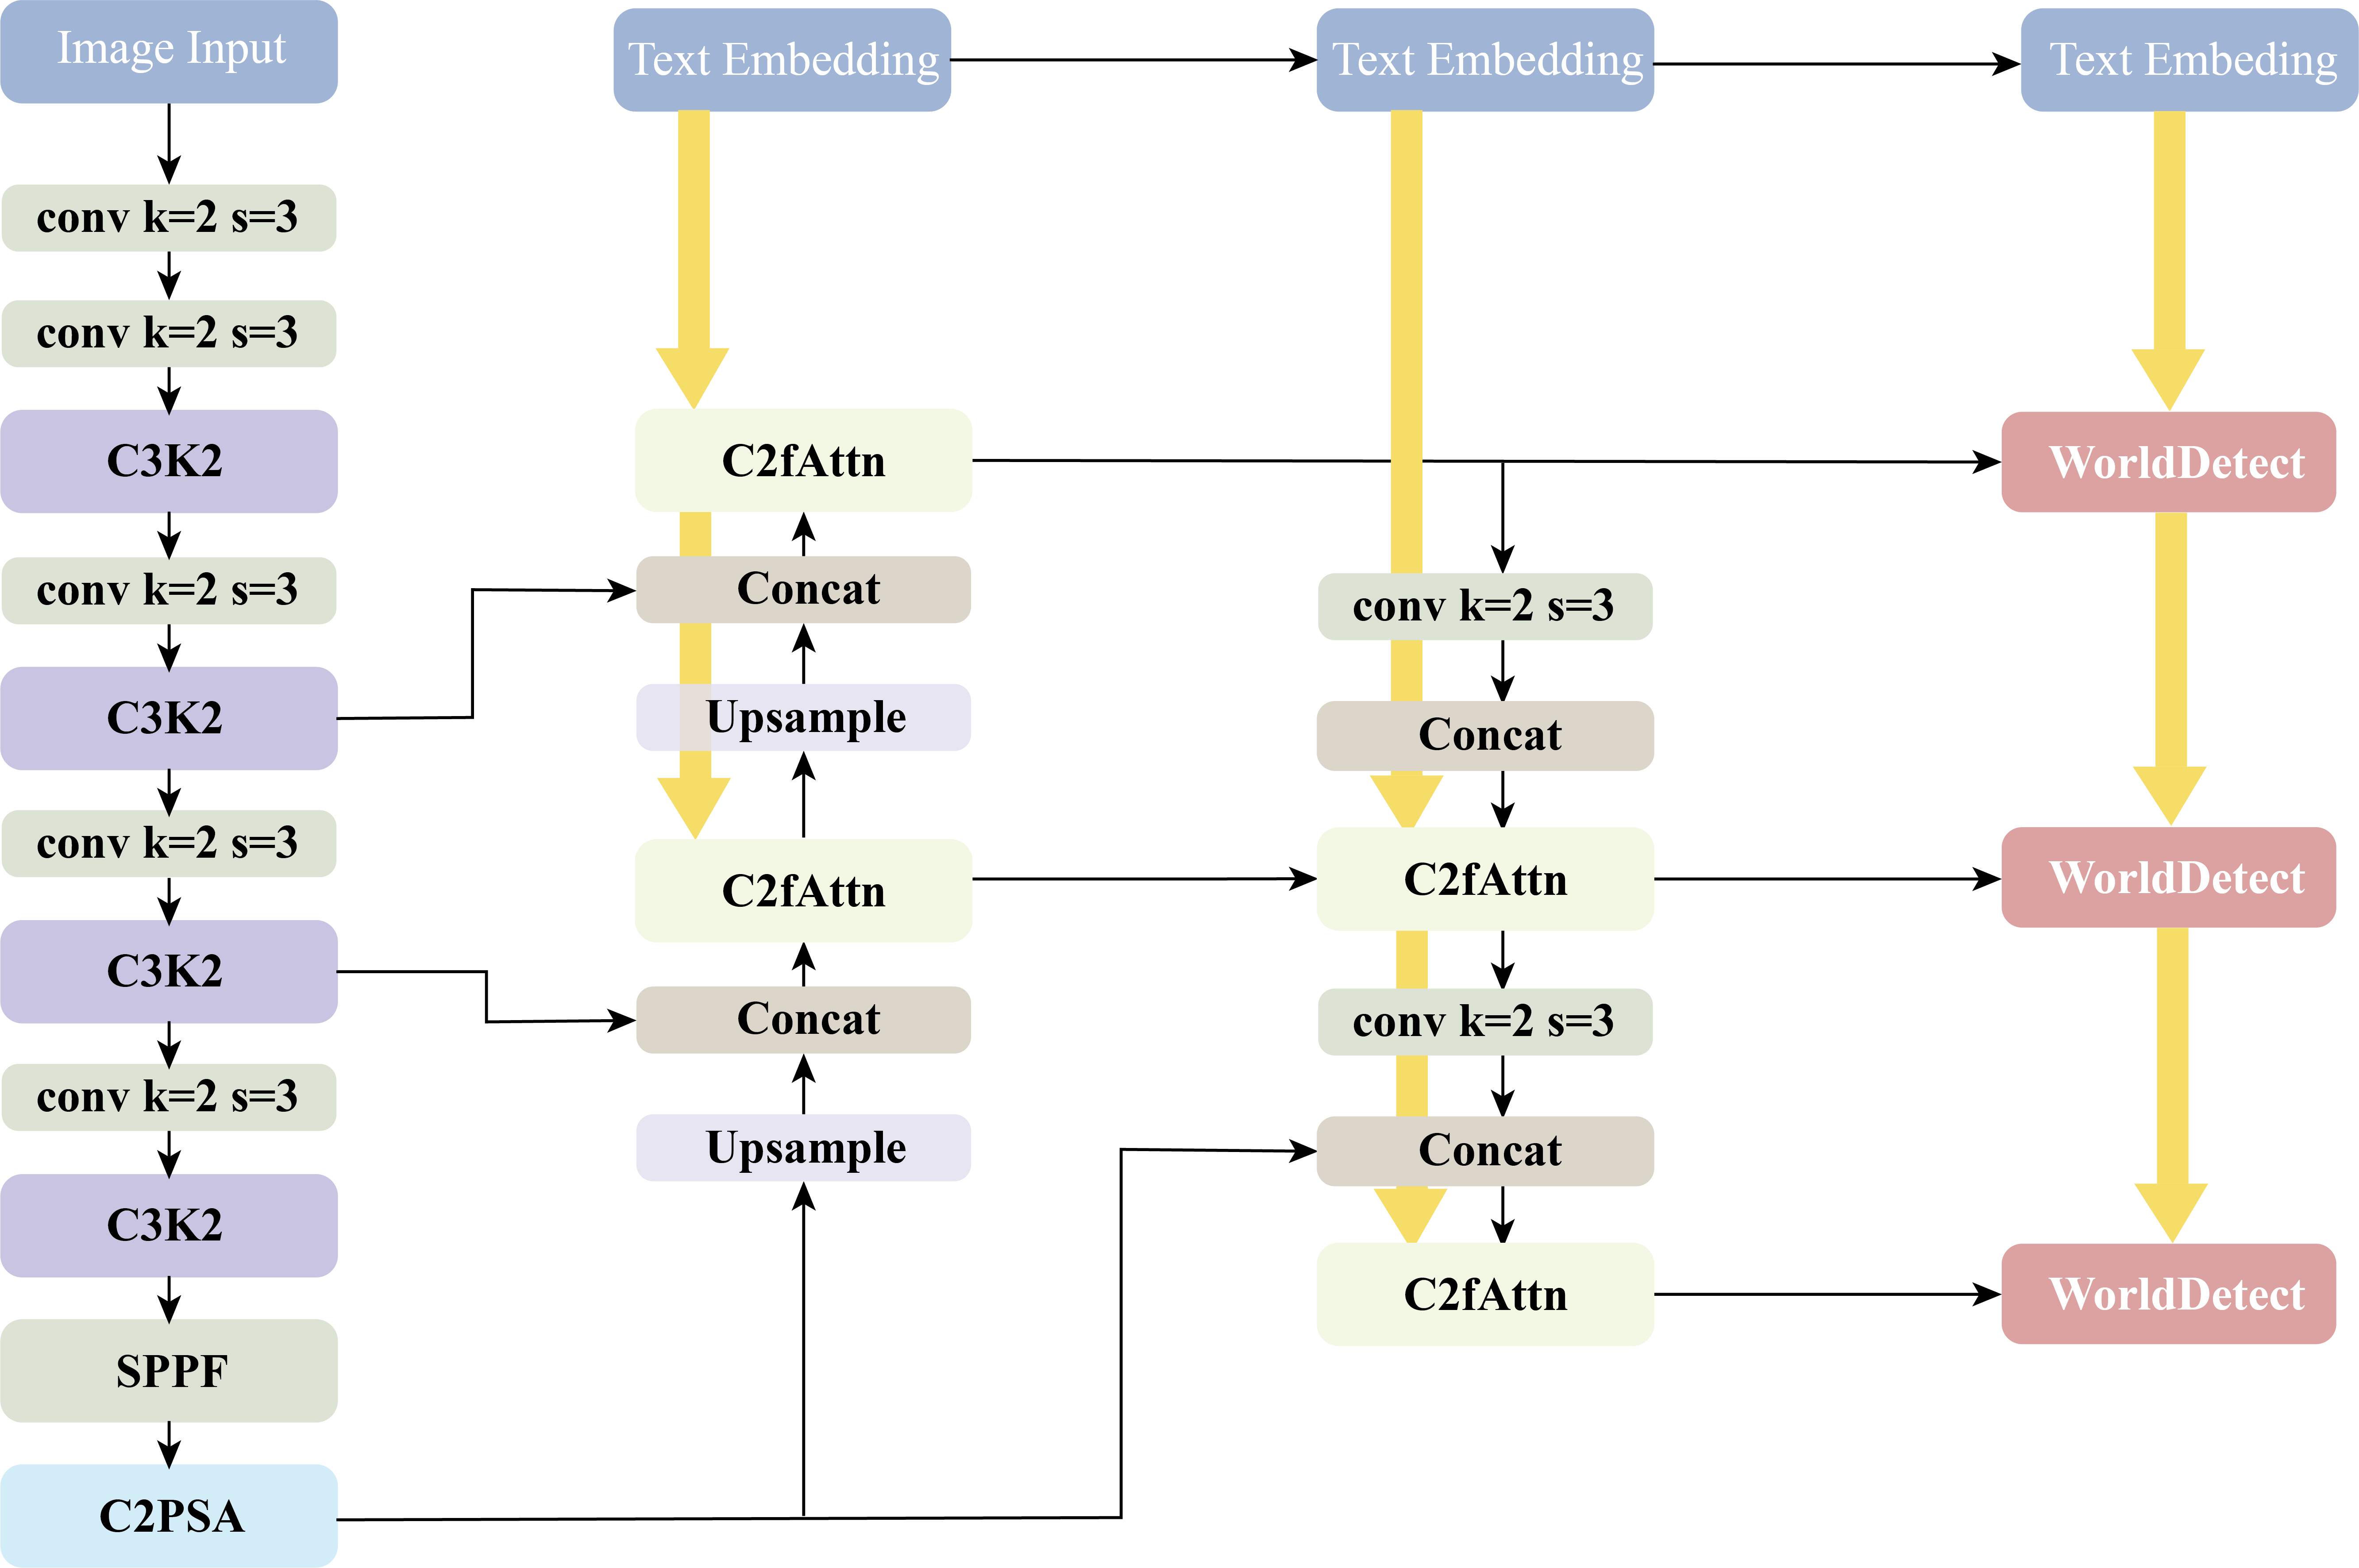
\includegraphics[width=10cm]{../image/4.png}
    \caption{The architecture of YOLO11-Earth. The model consists of a CSPNet backbone, a Vision-Language Path Aggregation Network (VL-PAN) for feature fusion, and a WorldDetect head for multi-modal detection. Text features from the CLIP text encoder are integrated at multiple levels of the network.}
    \label{fig:yolo11-earth-architecture}
\end{figure}
The YOLO11 model family’s greatest contribution lies in the use of the C3K2 module to achieve greater depth  
while maintaining gradient flow and fewer parameters compared to YOLOv8 (and even slightly better precision  
and speed on COCO compared to YOLOv9 and YOLOv10).

In simple terms, YOLO11-Earth can be seen as either:  
    1.A YOLO-Worldv2 model updated with a new backbone network and trained on a small closed-set multi-modal scheme,  
    2.A YOLO11 model endowed with new multi-modal learning capabilities, retrained on remote-sensing benchmarks  
         and adapted to application scenarios very different from YOLO-Worldv2.

This study uses the Ultralytics PyTorch implementation of YOLOv8-Worldv2, which is easier to deploy and train.  
Apart from the non-reparameterizable VL-PAN part, it is identical to the mmcv-based YOLO-Worldv2 and shares  
the same pretrained weights.

We denote model scales by appending s, m, l, or x to the version number (e.g., YOLO11s-Earth, YOLOv8x-Worldv2).

Figure 4 shows the detailed internal parameter layers of YOLO11-Earth.

\subsubsection{VL-PAN Design for Closed Sets}
The original YOLO-World architecture includes a
language–image alignment module that cannot be
deployed on consumer-grade GPUs. Although this
module can maximize the interaction between text
and image information, it consumes a significant
amount of computational resources. Therefore,
we prune this part.

Meanwhile, since the labels in xView are
hard-encoded (fixed text descriptions), we cannot
train text embeddings or classification heads.
Removing this part and retaining text features as
inputs to the model’s neck is a natural choice.

Thus, we adjust the RepVL-PAN
(Reparameterizable Vision-Language Path
Aggregation Network) in YOLO-Worldv2, retaining
the T-CSP block (mainly composed of C2FAttn modules)
as part of the YOLO model’s neck and removing the
original text embedding component for language–image
contrastive learning to complete the pruning. 
As shown in Figure 5, after aggregating text encoding
into image features, YOLO11-Earth does not update the text
encoding.

Finally, we add a step to feed text encoding into
the detection head, enabling it to perceive information
from both modalities and improve cross-dataset
transfer capabilities.

\begin{figure}[htbp]
    \centering
    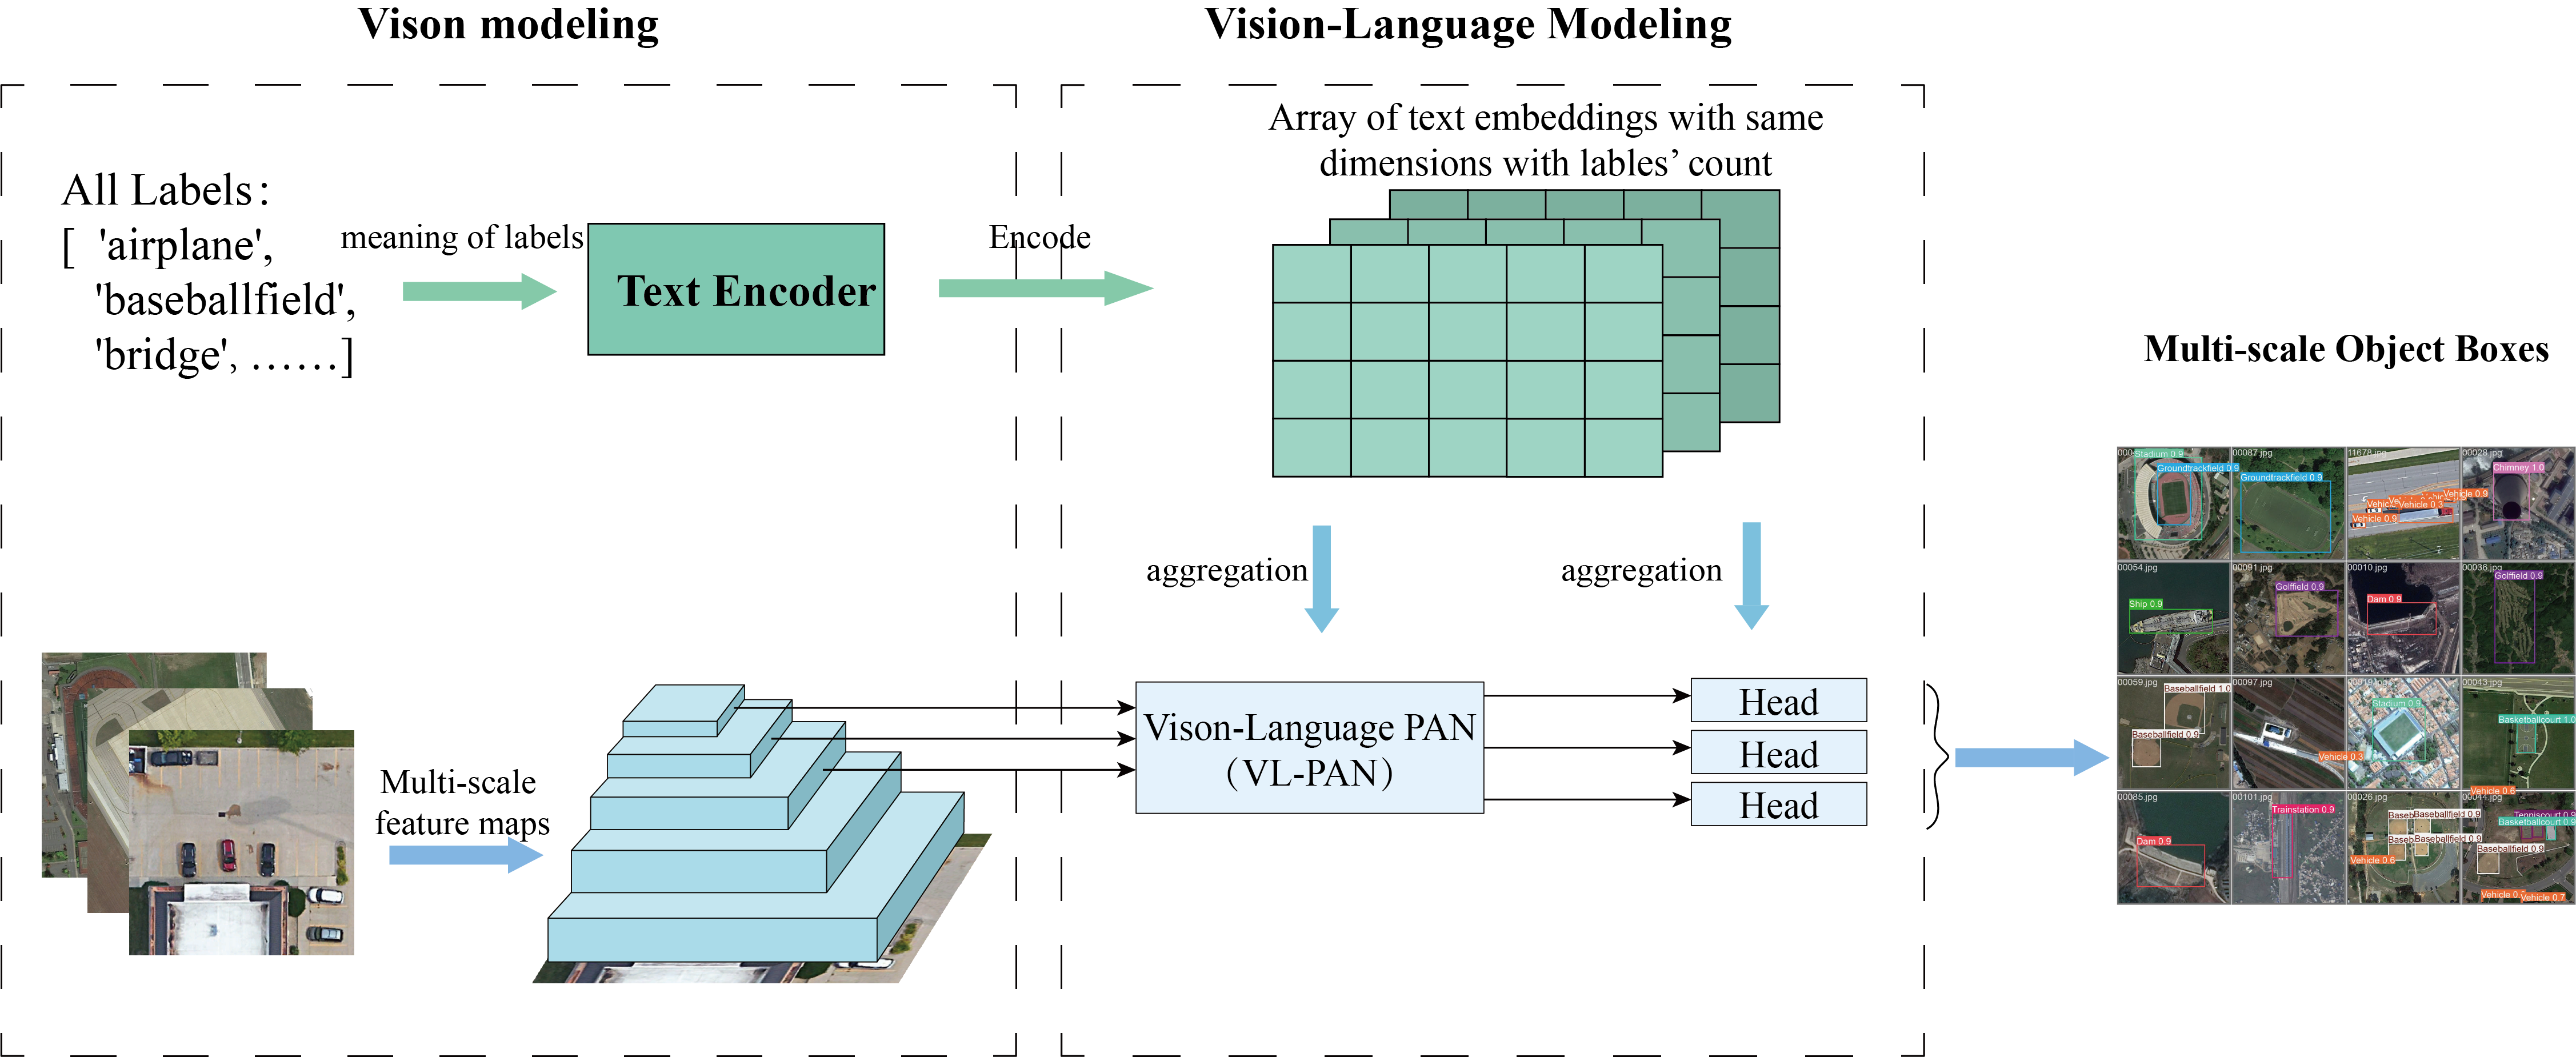
\includegraphics[width=12cm]{../image/5.png}
    \caption{Multi-Modal workflow of YOLO11-Earth. The model aggregate the text embeddings into the image features at multiple levels. The text features are encoded once and passed through the network as a feature supplement to the traditional YOLO11 model.}
\end{figure}

Overall, the redesigned VL-PAN (Vision-Language Path Aggregation Network)
no longer updates and forwards text encoding or calculates losses.
It only encodes all input label texts once and passes them through the network
as a feature supplement to the traditional YOLO model. This text feature can
be encoded once by CLIP (the chosen text encoder) during each training iteration
and stored, significantly reducing the model’s actual computational complexity.
Additionally, we no longer require a special text embedding loss function but
can directly apply the YOLO11 training loss, which consists of three parts:
bounding box loss, classification loss, and DFL (Distribution Focal Loss).

It is worth noting that since the semantic alignment module in YOLO-Worldv2 does
not participate in the forward process during inference (offline vocabulary mechanism),
we can still load its pre-trained weights published in the paper for ablation experiments
on the DIOR test set.

In summary, the VL-PAN design in YOLO11-Earth effectively integrates text features into the
image feature extraction process, enhancing the model’s ability to generalize across
different datasets while maintaining computational efficiency. This design choice
allows YOLO11-Earth to leverage the benefits of multi-modal learning without the prohibitive
computational costs associated with more complex language-image alignment modules.

\subsection{Pretraining on Closed-set Datasets}
\begin{figure}[htbp]
    \centering
    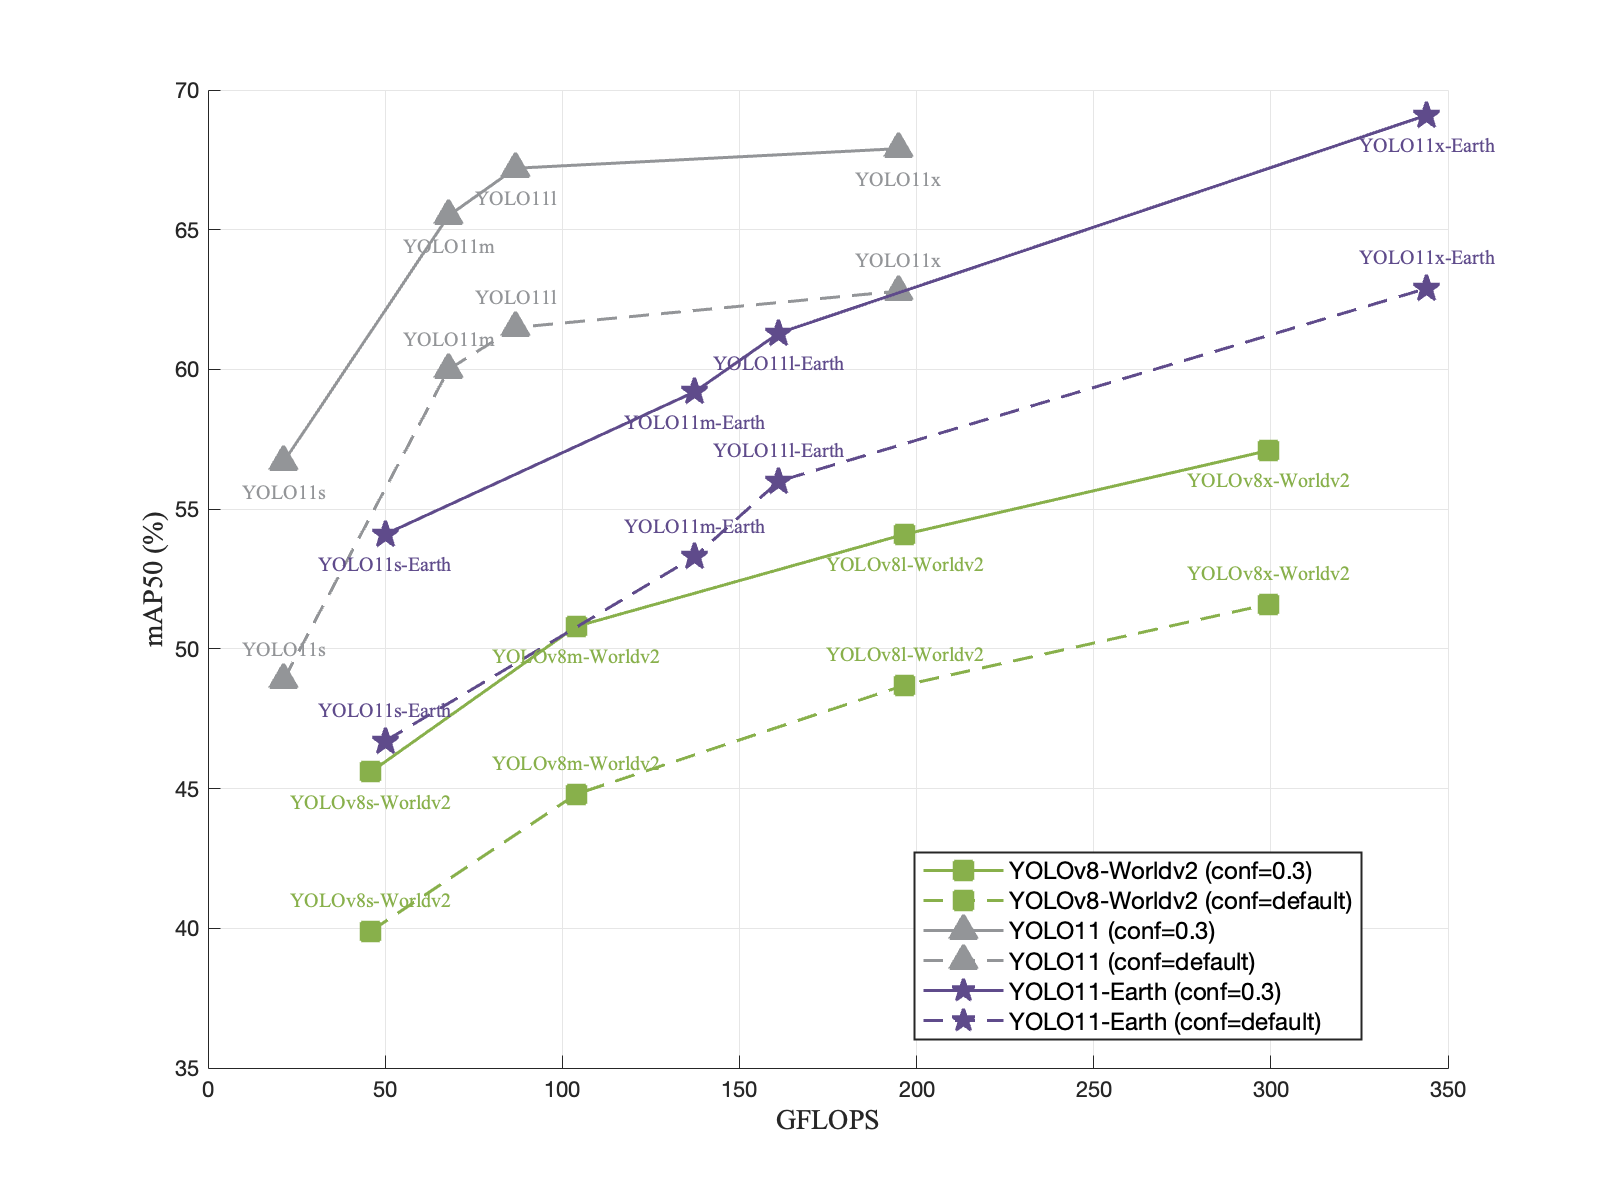
\includegraphics[width=10cm]{../image/6.png}
    \caption{Pretraining results of YOLO11-Earth and baseline models on xView-valid.}
\end{figure}
Table 1 presents the evaluation results of the 12 models across three model families on the validation set. 
On the xView validation set, we found that the pre-trained YOLO11-Earth significantly outperformed the 
YOLOv8-Worldv2 model trained on the same dataset and nearly matched the closed-set object detector YOLO11, 
which was also fully trained. During the precision assessment of the pre-trained models, 
we observed that the YOLO-World architecture (YOLOv8-Worldv2 and YOLO11-Earth) tended to detect more false 
positives (small targets with low confidence) in the validation set. However, by setting a lower confidence 
threshold, the precision of bounding boxes could be significantly improved, indicating that our models might 
overly focus on fine-grained features, leading to incorrect target detection in the background. Figure 6 more 
intuitively displays the performance differences among the three model families shown in Table 1. The use of a 
conf=0.3 filtering operation improved the mAP50 metric for all 12 models. Therefore, in subsequent experiments 
(including DIOR), we set the confidence threshold for evaluation tasks to conf=0.3. In addition to the performance 
boost brought by conf=0.3, Figure 6 also shows that YOLO11, as a single-modal model, exhibits lower inference costs.

Compared with YOLO11-Earth and YOLOv8-Worldv2, this performance difference implies that the improved backbone 
network has led to the performance gains of YOLO11-Earth. Directly using remote sensing images for pretraining 
offers the advantage of better approximating the model's global optimal parameters. Especially when comparing 
YOLOv8l-worldv2 with YOLO11m-worldv2, the latter, with 40\% fewer parameters, significantly outperforms the former, 
which roughly reflects the original performance difference between the YOLOv8 and YOLO11 series. This indicates 
that YOLO11-Earth has effectively inherited the feature extraction advantages of YOLO11. Compared with the 
closed-set detector YOLO11, YOLO11-Earth is significantly weaker in the s, m, and l sizes. This gap suggests 
that although the C2FAttn module acquires multimodal learning capabilities through attention mechanisms, 
it sacrifices a considerable portion of the pure image feature fitting capability compared to the C3K2 module. 
However, YOLO11x-Earth, by employing a larger parameter count, not only matches the object detection capability 
of YOLO11x but also gains the multimodal fusion capability absent in the closed-set detector (Table 1). This 
implies that the open vocabulary detection architecture typically requires a larger parameter count to balance 
the computation tasks of semantic and image features. As the parameter count increases, the model's ability to fit 
complex data distributions may improve.
\begin{table}[ht]
\centering
\caption{Metrics of YOLO11-Earth and baseline models on xView. In parentheses is the change of indicator relative to conf=default after conf=0.3 is used.}
\begin{tabular}{lcccccc}
\toprule
\textbf{Model Structure} & \textbf{P} & \textbf{R} & \textbf{mAP50} & \textbf{mAP50:95} & \textbf{GFLOPS} & \textbf{Parameters} \\
\midrule
YOLOv8s-Worldv2 & 52.1 (+0.5) & 36.5 (-6.5) & 45.6 (+5.7) & 29.2 (+5.4) & 46 & 12,749,288 \\
YOLOv8m-worldv2 & 55.9 (-0.9) & 42.1 (+0.22) & 50.8 (+6) & 33.3 (+5.8) & 103.9 & 28,358,830 \\
YOLOv8l-Worldv2 & 57.9 (-0.5) & 46.1 (-1.7) & 54.1 (+5.4) & 36.3 (+5.7) & 196.6 & 46,807,922 \\
YOLOv8x-Worldv2 & 59.4 (-1.2) & 49.7 (+0) & 57.1 (+5.5) & 38.7 (+5.7) & 299.4 & 72,856,217 \\
\midrule
YOLO11s-Earth & 65.4 (+7.1) & 40.4 (-5.9) & 54.1 (+7.4) & 36.2 (+7.2) & 50.0 & 15,173,752 \\
YOLO11m-Earth & 64.2 (-1.0) & 49.4 (-1.0) & 59.2 (+5.9) & 41.0 (+6.2) & 137.4 & 33,155,954 \\
YOLO11l-Earth & 63.6 (-0.4) & 53.2 (-0.8) & 61.3 (+5.3) & 43.0 (+5.7) & 161.1 & 39,894,386 \\
YOLO11x-Earth & 73.4 (+1.8) & 58.1 (-0.9) & 69.1 (+6.2) & 51.8 (+7.2) & 344.0 & 89,081,536 \\
\midrule
YOLO11s & 68.4 (+6.2) & 42.5 (-5.5) & 56.7 (+7.8) & 38.1 (+7.6) & 21.4 & 9,436,020 \\
YOLO11m & 71.8 (+0) & 54.5 (-0.6) & 65.5 (+5.5) & 46.4 (+6.3) & 67.9 & 20,076,292 \\
YOLO11l & 71.2 (+0.3) & 57.9 (-0.1) & 67.2 (+5.7) & 47.7 (+6.5) & 86.8 & 25,325,572 \\
YOLO11x & 72.2 (-1.8) & 58.3 (+0.1) & 67.9 (+5.1) & 49.0 (+6.0) & 194.8 & 56,896,324 \\
\bottomrule
\end{tabular}
\end{table}
To test whether our block strategy, in addition to reducing GPU runtime pressure, can improve the model's ability 
to perceive small targets in large-size images, we evaluated the block-pretrained models on the original-size 
xView validation set. The performance metrics are shown in Table 2. The results indicate that even though the 
models were trained on block images, all our open vocabulary detection models could still perform efficient 
$1024 \times 1024$ inference on the original validation set and achieve performance comparable to state-of-the-art 
models. However, since our sub-images might contain partial information from the original validation set and the 
mAP50 metric is relatively more lenient than the mAP metric, we cannot conclude that our models have surpassed the 
MTP model's performance [49]. Nevertheless, this performance demonstrates that training on block images can 
enhance the model's inference effects on larger input images. This improvement originates from the model 
parameters' fitting to finer-grained features and the repeated learning of difficult targets due to overlapping 
sub-images. This also corroborates the effectiveness of the SF method and the corresponding SAHI method for small 
target detection in very large images. Although our training and inference did not directly use the SAHI library, 
the principles are essentially the same.
\begin{table}[ht]
\centering
\caption{Metrics of YOLO11-Earth and baseline models on the original-size xView validation set.}
\begin{tabular}{lcccccc}
\toprule
\textbf{Model Structure} & \textbf{P} & \textbf{R} & \textbf{mAP50} & \textbf{mAP50:95} & \textbf{GFLOPS} & \textbf{Parameters} \\
\midrule
YOLOv8s-Worldv2 & 21.0 & 3.75 & 12.3 & 7.40 & 46 & 12,749,288 \\
YOLOv8m-Worldv2 & 26.1 & 6.20 & 15.9 & 8.73 & 103.9 & 28,358,830 \\
YOLOv8l-Worldv2 & 27.4 & 6.87 & 17.1 & 9.89 & 196.6 & 46,807,922 \\
YOLOv8x-Worldv2 & 35.2 & 7.60 & 21.1 & 11.90 & 299.4 & 72,856,217 \\
\midrule
YOLO11s-Earth & 26.7 & 6.15 & 16.1 & 9.85 & 50.0 & 15,173,752 \\
YOLO11m-Earth & 32.6 & 7.73 & 20.3 & 11.60 & 137.4 & 33,155,954 \\
YOLO11l-Earth & 34.7 & 8.73 & 21.5 & 11.60 & 161.1 & 39,894,386 \\
YOLO11x-Earth & 36.7 & 9.31 & 22.9 & 13.90 & 344.0 & 89,081,536 \\
\bottomrule
\end{tabular}
\end{table}
Even though the models were trained on block images, all our open vocabulary detection models could still perform 
efficient $1024 \times 1024$ inference on the original validation set and achieve performance comparable to 
state-of-the-art models. However, since our sub-images might contain partial information from the original 
validation set and the mAP50 metric is relatively more lenient than the mAP metric, we cannot conclude that 
our models have surpassed the MTP model's performance \cite{wang2024mtp}. Nevertheless, this performance demonstrates that 
training on block images can enhance the model's inference effects on larger input images. This improvement 
originates from the model parameters' fitting to finer-grained features and the repeated learning of difficult 
targets due to overlapping sub-images. This also corroborates the effectiveness of the SF method and the 
corresponding SAHI method for small target detection in very large images. Although our training and inference 
did not directly use the SAHI library, the principles are essentially the same.
\subsection{Cross-dataset Transfer Results}
\subsubsection{Zero-Shot Transfer Results}
Table 3 shows the performance comparison of YOLO11-Earth and baseline models on the DIOR test set for zero-shot 
transfer. To evaluate the zero-shot transfer capabilities of our open vocabulary detector on an unseen dataset, 
we used the 12 pre-trained models from Section 5.1, as well as the pre-trained weights of YOLOv8-Worldv2 from its 
paper, and conducted inference and evaluation on the DIOR test set by merely modifying the vocabulary.

\begin{table}[ht]
\centering
\caption{Metrics of YOLO11-Earth and baseline models on the DIOR test set for zero-shot transfer.}
\begin{tabular}{lcccccc}
\toprule
\textbf{Model Structure} & \textbf{P} & \textbf{R} & \textbf{mAP50} & \textbf{mAP50:95} & \textbf{GFLOPS} \\
\midrule
YOLOv8s-Worldv2 & 7.74\% & 11.5\% & 8.12\% & 3.67\% & 46 \\
YOLOv8m-Worldv2 & 7.87\% & 11.9\% & 8.11\% & 2.98\% & 103.9 \\
YOLOv8l-Worldv2 & 7.87\% & 11.9\% & 8.11\% & 2.98\% & 196.6 \\
YOLOv8x-Worldv2 & 10.40\% & 15.6\% & 9.95\% & 3.57\% & 299.4 \\
\midrule
YOLOv8s-Worldv2 (untrained on xView) & 10.30\% & 2.62\% & 2.10\% & 1.06\% & 51.0 \\
YOLOv8m-Worldv2 (untrained on xView) & 38.20\% & 2.10\% & 3.27\% & 1.85\% & 110.5 \\
YOLOv8l-Worldv2 (untrained on xView) & 27.90\% & 3.03\% & 3.49\% & 1.92\% & 204.5 \\
YOLOv8x-Worldv2 (untrained on xView) & 14.60\% & 4.64\% & 4.49\% & 2.51\% & 309.3 \\
\midrule
YOLO11s-Earth & 8.20\% & 6.09\% & 6.26\% & 2.98\% & 50.0 \\
YOLO11m-Earth & 10.40\% & 7.72\% & 7.79\% & 3.92\% & 137.4 \\
YOLO11l-Earth & 10.20\% & 7.23\% & 7.15\% & 3.47\% & 161.1 \\
YOLO11x-Earth & 12.90\% & 3.92\% & 7.95\% & 4.35\% & 344.0 \\
\midrule
YOLOv11s & - & - & - & - & 21.4 \\
YOLOv11m & - & - & - & - & 67.9 \\
YOLOv11l & - & - & - & - & 86.8 \\
YOLOv11x & - & - & - & - & 194.8 \\
\bottomrule
\end{tabular}
\end{table}
The results indicate that pretraining on the xView dataset significantly enhances the zero-shot transfer 
capabilities of the open vocabulary detection models on remote sensing images. Comparing the YOLOv8-Worldv2 
models trained with and without xView, it is evident that including remote sensing images in the training set 
greatly improves the model's ability to generalize to new datasets. However, YOLO11-Earth, despite its superior 
performance during pretraining, exhibits slightly weaker zero-shot capabilities on the DIOR dataset compared to 
YOLOv8-Worldv2. This discrepancy may arise from the closed-set training data's inability to enforce alignment 
between language and image features, leading to an overemphasis on image features. Meanwhile, the closed-set 
single-modal detector YOLO11 completely lacks open vocabulary detection capabilities. For instance, YOLO11s 
achieved an mAP50 of 58.9\% on the first label, 0.66\% on the 14th label, and 0.45\% on the 19th label, with 
zero precision for the remaining labels. This inconsistent performance demonstrates that YOLO11 cannot reliably 
classify objects in the DIOR dataset, as the labels it learned from xView do not match those in DIOR.
\subsubsection{Full Fine-tuning Transfer Results}
\begin{figure}[htbp]
    \centering
    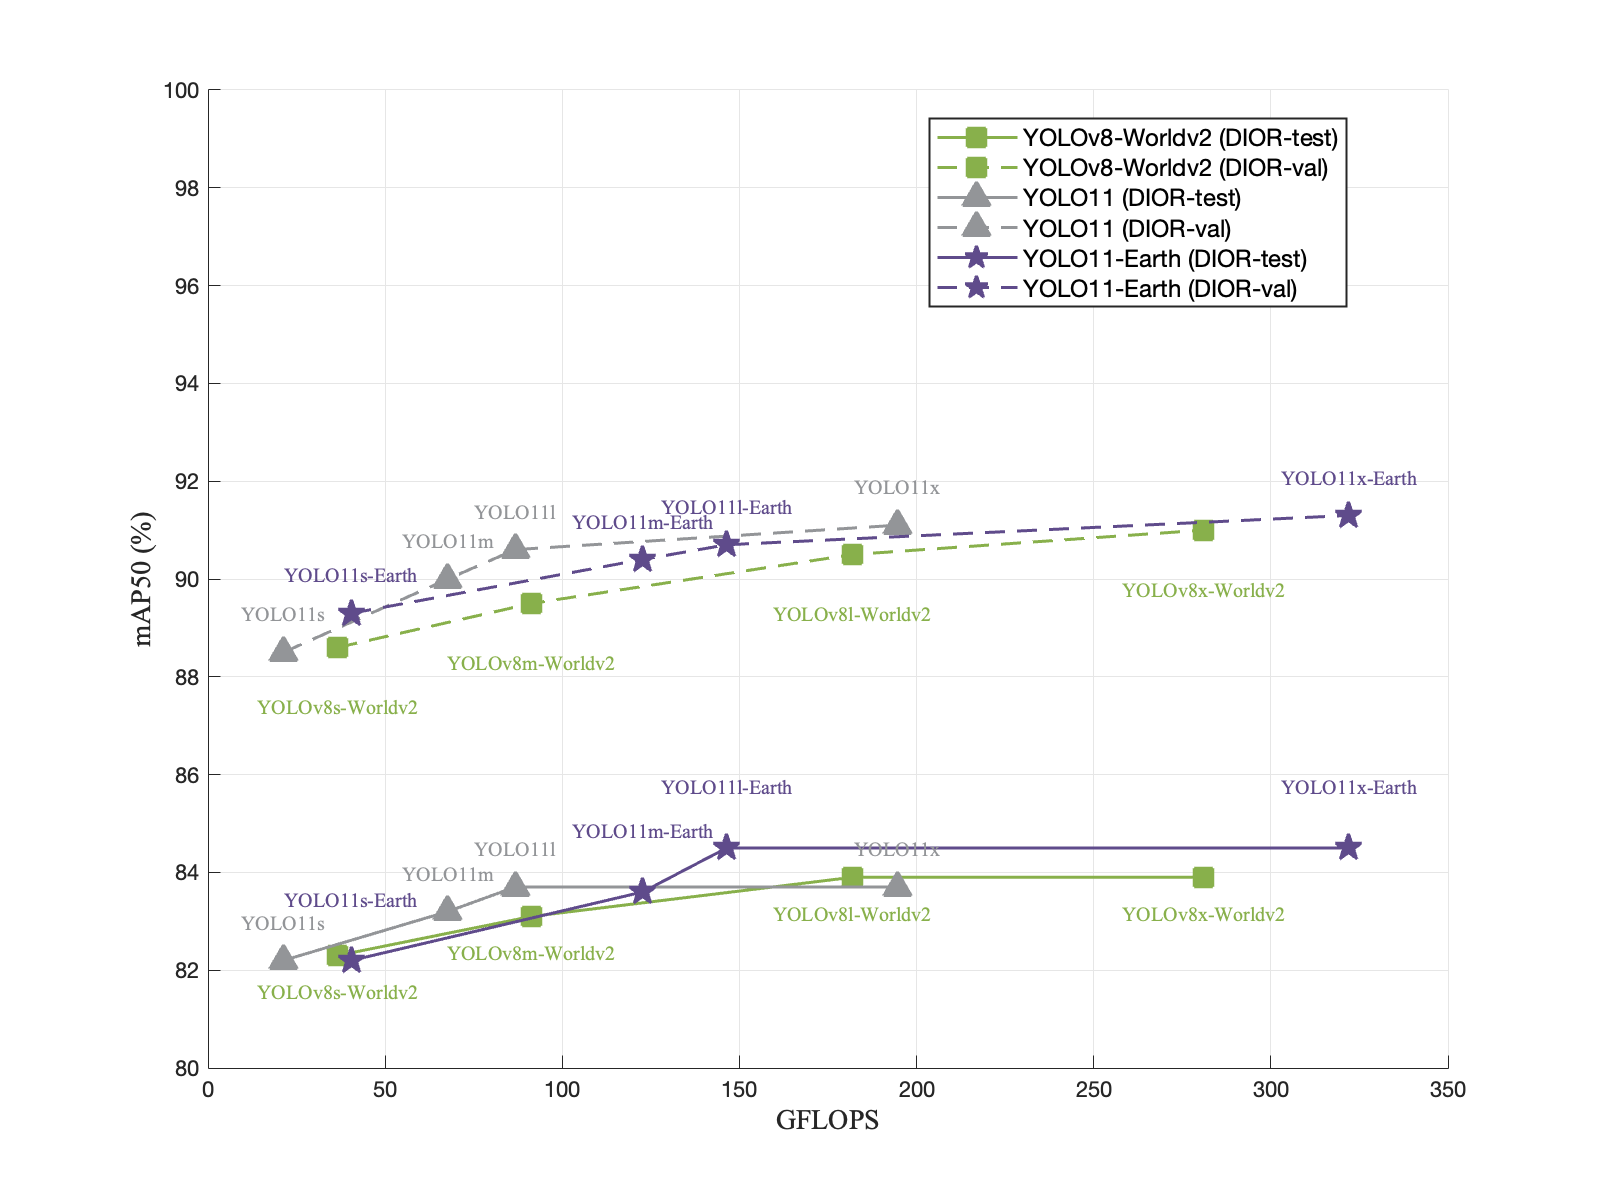
\includegraphics[width=10cm]{../image/7.png}
    \caption{Fine-tuning with full train set results of YOLO11-Earth and baseline models on DIOR.}
\end{figure}
After the zero-shot transfer experiments, we conducted fine-tuning experiments using the complete training set 
(DIOR-train) for all 12 models. In this scenario, the open vocabulary detectors and the traditional closed-set 
detectors perform the same task, and we aim to verify whether the open vocabulary detectors with semantic 
information can achieve learning with fewer training iterations (80–120 iterations with early stopping).

Table 4 shows the performance metrics of the pre-trained models on the validation and test sets after 
fine-tuning on the DIOR dataset. Figure 7 provides a more intuitive comparison of the models' performance.
\begin{table}[ht]
\centering
\caption{Metrics of YOLO11-Earth and baseline models on the DIOR validation and test sets after full fine-tuning.}
\begin{tabular}{lcccccc}
\toprule
\textbf{Model Structure} & \textbf{mAP50-val} & \textbf{mAP50:95-val} & \textbf{mAP50-test} & \textbf{mAP50:95-test} & \textbf{GFLOPS} \\
\midrule
YOLOv8s-Worldv2 & 88.6\% & 69.4\% & 82.3\% & 64.3\% & 36.6 \\
YOLOv8m-Worldv2 & 89.5\% & 72.3\% & 83.1\% & 66.2\% & 91.3 \\
YOLOv8l-Worldv2 & 90.5\% & 73.5\% & 83.9\% & 67.0\% & 181.9 \\
YOLOv8x-Worldv2 & 91.0\% & 74.0\% & 83.9\% & 67.3\% & 281.1 \\
\midrule
YOLO11s-Earth & 89.3\% & 71.1\% & 82.2\% & 64.8\% & 50.0 \\
YOLO11m-Earth & 90.4\% & 71.6\% & 83.6\% & 65.5\% & 122.7 \\
YOLO11l-Earth & 90.7\% & 72.7\% & 84.5\% & 66.8\% & 161.1 \\
YOLO11x-Earth & 91.3\% & 74.2\% & 84.5\% & 67.2\% & 322.0 \\
\midrule
YOLO11s & 85.5\% & 69.6\% & 82.2\% & 64.4\% & 21.3 \\
YOLO11m & 90.0\% & 72.2\% & 83.2\% & 65.7\% & 67.7 \\
YOLO11l & 90.6\% & 73.9\% & 83.7\% & 66.9\% & 86.7 \\
YOLO11x & 91.1\% & 74.3\% & 83.7\% & 67.1\% & 194.5 \\
\bottomrule
\end{tabular}
\end{table}

\begin{table}[ht]
\centering
\caption{Comparison of YOLO11-Earth with state-of-the-art models on the DIOR test set.}
\resizebox{\textwidth}{!}{%
\begin{tabular}{lccc}
\toprule
\textbf{Model Structure} & \textbf{Backbone Network} & \textbf{Pretraining Data} & \textbf{mAP50-test (\%)} \\
\midrule
\multicolumn{4}{l}{\textit{General Object Detection Models}} \\
\midrule
GASSL \cite{ayush2021geography} & ResNet-50 & - & 67.40 \\
CACO \cite{mall2023change} & ResNet-50 & Sentinel-2 & 66.91 \\
TOV \cite{tao2023tov} & ResNet-50 & TOV-NI, TOV-R & 70.16 \\
Scale-MAE \cite{reed2023scale} & ViT-L & FMoW & 73.81 \\
SatLas \cite{bastani2023satlaspretrain} & Swin-B & SatlasPretrain & 74.10 \\
RingMo \cite{sun2022ringmo} & Swin-B & RingMoPretrain & 75.90 \\
SkySense \cite{guo2024skysense} & Swin-H & Multi-modal RSI & 78.73 \\
MTP \cite{wang2024mtp} & Swin-H & MillionAID & 81.10 \\
\midrule
\multicolumn{4}{l}{\textit{Open Vocabulary (Open Set) Detection Models}} \\
\midrule
GLIP-FT \cite{li2022grounded,pan2025locate} & Swin-H & O365, GoldG, CC3M, SBU & 87.8 \\
GroundingDINO-FT \cite{liu2024grounding,pan2025locate}& Swin-H & O365, GoldG, Cap4M & 90.4 \\
GroundingDINO-FT \cite{liu2024grounding,pan2025locate} & Swin-H & LAE-1M & 91.1 \\
LAE-DINO-FT \cite{pan2025locate} & Swin-H & O365, GoldG, Cap4M & 92.0 \\
LAE-DINO-FT \cite{pan2025locate} & Swin-H & LAE-1M & 92.2 \\
YOLO11x-Earth (proposed) & CSPNet & xView & 84.5 \\
\bottomrule
\end{tabular}%
}
\end{table}

The results demonstrate that YOLO11-Earth, based on YOLO11 and YOLOv8-Worldv2, 
is a successful practice of promoting closed-set detectors to open vocabulary detection. 
An important finding is that after fine-tuning, the computational cost (GFLOPS) of the two open 
vocabulary models dropped significantly, while the parameter reduction in YOLO11 was minimal. 
This difference is likely due to the DIOR dataset having shorter labels and 40 fewer categories 
compared to the xView dataset. In the two open vocabulary detection models, labels are stored as 
text features, whereas in YOLO11, they correspond one-to-one with the fully connected layer's 
numerical mapping, as in most single-modal models.
\subsubsection{Less Data Fine-tuning Transfer Results}
Similar to LAE-DINO, to investigate the transfer learning capabilities of YOLO11-Earth under data scarcity 
conditions, we conducted fine-tuning experiments on the train-quarter and train-half datasets, which were 
randomly sampled from the full DIOR training set. 

YOLO11 exhibited the weakest performance among the three model families. Even with rich pre-trained weights, 
it struggled to converge quickly under data scarcity conditions. This indicates that single-modal models are 
more prone to falling into local optima when forced to converge rapidly compared to open vocabulary detectors. 
As expected, the multi-modal information learned by YOLO-Worldv2 and YOLO11-Earth facilitated quicker training 
and superior performance. However, there were differences in the ease of parameter convergence among the models. 
To ensure the significance of the ablation experiments, we did not repeatedly adjust the hyperparameters and 
used the same default settings for all models of the same size. Compared to YOLOv8-Worldv2, the two YOLO11-based 
networks were more prone to early stopping on the 25\% training dataset, resulting in slightly lower metrics for 
YOLO11-Earth. Nevertheless, YOLO11-Earth was relatively easier to train. The models' depth (number of parameter 
layers) was in the order of YOLO11-Earth, YOLO-Worldv2, and YOLO11, suggesting that training difficulty is 
proportional to the number of parameter layers, and additional modal information helps mitigate this difficulty.
When the training dataset size reached 50\%, YOLO11-Earth's performance advantage became more pronounced. 
The two multi-modal models were relatively easier to train, while YOLO11 still faced challenges in converging 
quickly and often terminated prematurely. At this dataset size, we observed that the l and x-sized models 
performed similarly on the DIOR test set, indicating that the 50\% DIOR training dataset was insufficient to 
support the x-sized model with over 70M parameters. Interestingly, larger models with more parameters did not 
necessarily outperform smaller models, as seen in the comparison between YOLO11x and YOLO11l. This suggests 
that optimizing a more complex non-linear mapping is challenging with a reduced training dataset size. This 
conclusion is supported by the performance on the larger and more challenging xView dataset, where we have 
demonstrated the scaling laws within each model family.

Table 6 provides a comprehensive comparison of the mAP50 dynamics for the models fine-tuned on different-sized training datasets. YOLO11-Earth consistently outperformed the other models on the test set across all three training scenarios (25\%, 50\%, and full training data), and matched YOLOv8-Worldv2 on the validation set. YOLOv8-Worldv2 showed good performance on the validation set but lagged on the test set. Meanwhile, YOLO11 struggled to leverage its architectural advantages under data scarcity and strict iteration limits, and could not compete with YOLO11-Earth and YOLOv8-Worldv2 even with advanced neck and head designs. This dynamic change highlights the contribution of the multi-modal input in open vocabulary detectors to the model's ability to quickly adapt to new datasets. Clearly, YOLO11-Earth inherited the cross-dataset rapid transfer capabilities similar to the YOLO-World architecture, especially when compared to YOLO11 under data scarcity conditions. This confirms that the pretraining phase of our lightweight OVD model indeed endows YOLO11-Earth with the corresponding capabilities.

\begin{table}[ht]
\centering
\caption{Model performance comparison with different training data sizes.}
\begin{tabular}{lcccccc}
\toprule
\multirow{2}{*}{\textbf{Model Structure}} & \multicolumn{2}{c}{\textbf{Train-Quarter}} & \multicolumn{2}{c}{\textbf{Train-Half}} & \multicolumn{2}{c}{\textbf{Train-Full}} \\
\cmidrule(lr){2-7}
 & mAP50-val & mAP50-test & mAP50-val & mAP50-test & mAP50-val & mAP50-test \\
\midrule
YOLOv8s-Worldv2 & 82.0\% & 75.0\% & 84.5\% & 77.9\% & 88.6\% & 82.3\% \\
YOLOv8m-Worldv2 & 85.0\% & 77.5\% & 85.3\% & 78.6\% & 89.5\% & 83.1\% \\
YOLOv8l-Worldv2 & 85.0\% & 77.6\% & 88.2\% & 81.1\% & 90.5\% & 83.9\% \\
YOLOv8x-Worldv2 & 85.6\% & 77.7\% & 88.6\% & 81.0\% & 91.0\% & 83.9\% \\
\midrule
YOLO11s-Earth   & 82.5\% & 75.6\% & 86.3\% & 78.8\% & 89.3\% & 82.2\% \\
YOLO11m-Earth   & 84.0\% & 76.7\% & 87.6\% & 80.7\% & 90.4\% & 83.6\% \\
YOLO11l-Earth   & 84.3\% & 77.3\% & 88.0\% & 81.1\% & 90.7\% & 84.5\% \\
YOLO11x-Earth   & 84.4\% & 77.7\% & 88.5\% & 81.3\% & 91.3\% & 84.5\% \\
\midrule
YOLO11s         & 78.2\% & 70.5\% & 84.0\% & 76.3\% & 85.5\% & 82.2\% \\
YOLO11m         & 81.2\% & 73.2\% & 87.1\% & 79.6\% & 90.0\% & 83.2\% \\
YOLO11l         & 83.8\% & 75.9\% & 88.4\% & 80.6\% & 90.6\% & 83.7\% \\
YOLO11x         & 83.2\% & 75.5\% & 88.3\% & 80.0\% & 91.1\% & 83.7\% \\
\bottomrule
\end{tabular}
\end{table}

\subsection{Cross-task Transfer Results}
To evaluate the cross-task transfer learning capabilities of YOLO11-Earth, we conducted experiments using the 
YOLO11-seg model initialized with the pre-trained YOLO11-Earth backbone network on the Potsdam segmentation 
dataset. Specifically, we fine-tuned the YOLO11-seg model with and without freezing the backbone network to 
assess the segmentation performance on the Potsdam dataset.

Table 7 presents the performance metrics of the YOLO11-seg model fine-tuned with the YOLO11-Earth weights on the Potsdam dataset.
\begin{table}[ht]
\centering
\caption{Performance metrics of the YOLO11-seg model on the Potsdam dataset.}
\begin{tabular}{lccccc}
\toprule
\textbf{Model} & \textbf{P} & \textbf{R} & \textbf{mAP50} & \textbf{mAP50:95} & \textbf{Best at(epochs)} \\
\midrule
YOLO11s-Earth (Frozen) & 68.9\% & 56.1\% & 65.7\% & 45.1\% & 42 \\
YOLO11m-Earth (Frozen) & 71.8\% & 59.0\% & 68.3\% & 47.6\% & 58 \\
YOLO11l-Earth (Frozen) & 73.4\% & 59.5\% & 69.0\% & 48.8\% & 52 \\
YOLO11x-Earth (Frozen) & 72.3\% & 61.1\% & 69.4\% & 49.9\% & 49 \\
YOLO11s-Earth (Unfrozen) & 72.0\% & 62.1\% & 70.2\% & 49.6\% & 60 \\
YOLO11m-Earth (Unfrozen) & 74.2\% & 63.8\% & 71.9\% & 51.6\% & 48 \\
YOLO11l-Earth (Unfrozen) & 75.7\% & 63.8\% & 72.3\% & 53.0\% & 55 \\
YOLO11x-Earth (Unfrozen) & 76.1\% & 63.7\% & 72.7\% & 53.8\% & 38 \\
\bottomrule
\end{tabular}
\end{table}
The results indicate that the pre-trained backbone network of YOLO11-Earth significantly enhanced the convergence 
speed of the YOLO11-seg model on the Potsdam dataset, regardless of whether the backbone network was frozen or 
not. When the backbone network was frozen, the model achieved reasonable segmentation performance with fewer 
iterations, demonstrating the effectiveness of the pre-trained weights as a strong prior for the segmentation 
task. When the backbone network was unfrozen, allowing the weights to be updated during fine-tuning, the 
segmentation performance further improved, indicating that the pre-trained backbone network could adapt to 
the new task and dataset.

Figure 8 illustrates the segmentation results of the YOLO11x-Earth fine-tuned YOLO11x-seg model on the test set of the Potsdam dataset. The segmentation results were visualized by converting the bounding box predictions back to masks using RGB mapping. The model showed good performance in segmenting objects with relatively fixed shapes, such as trees and cars. However, for objects with more diverse shapes, such as impervious surfaces, sparse vegetation, and buildings, the segmentation accuracy was lower. This is partly due to the design of the Potsdam dataset, which includes a background class that leads to significant overlap of bounding boxes, making it challenging to achieve accurate pixel-level instance segmentation.
\begin{figure}[htbp]
    \centering
    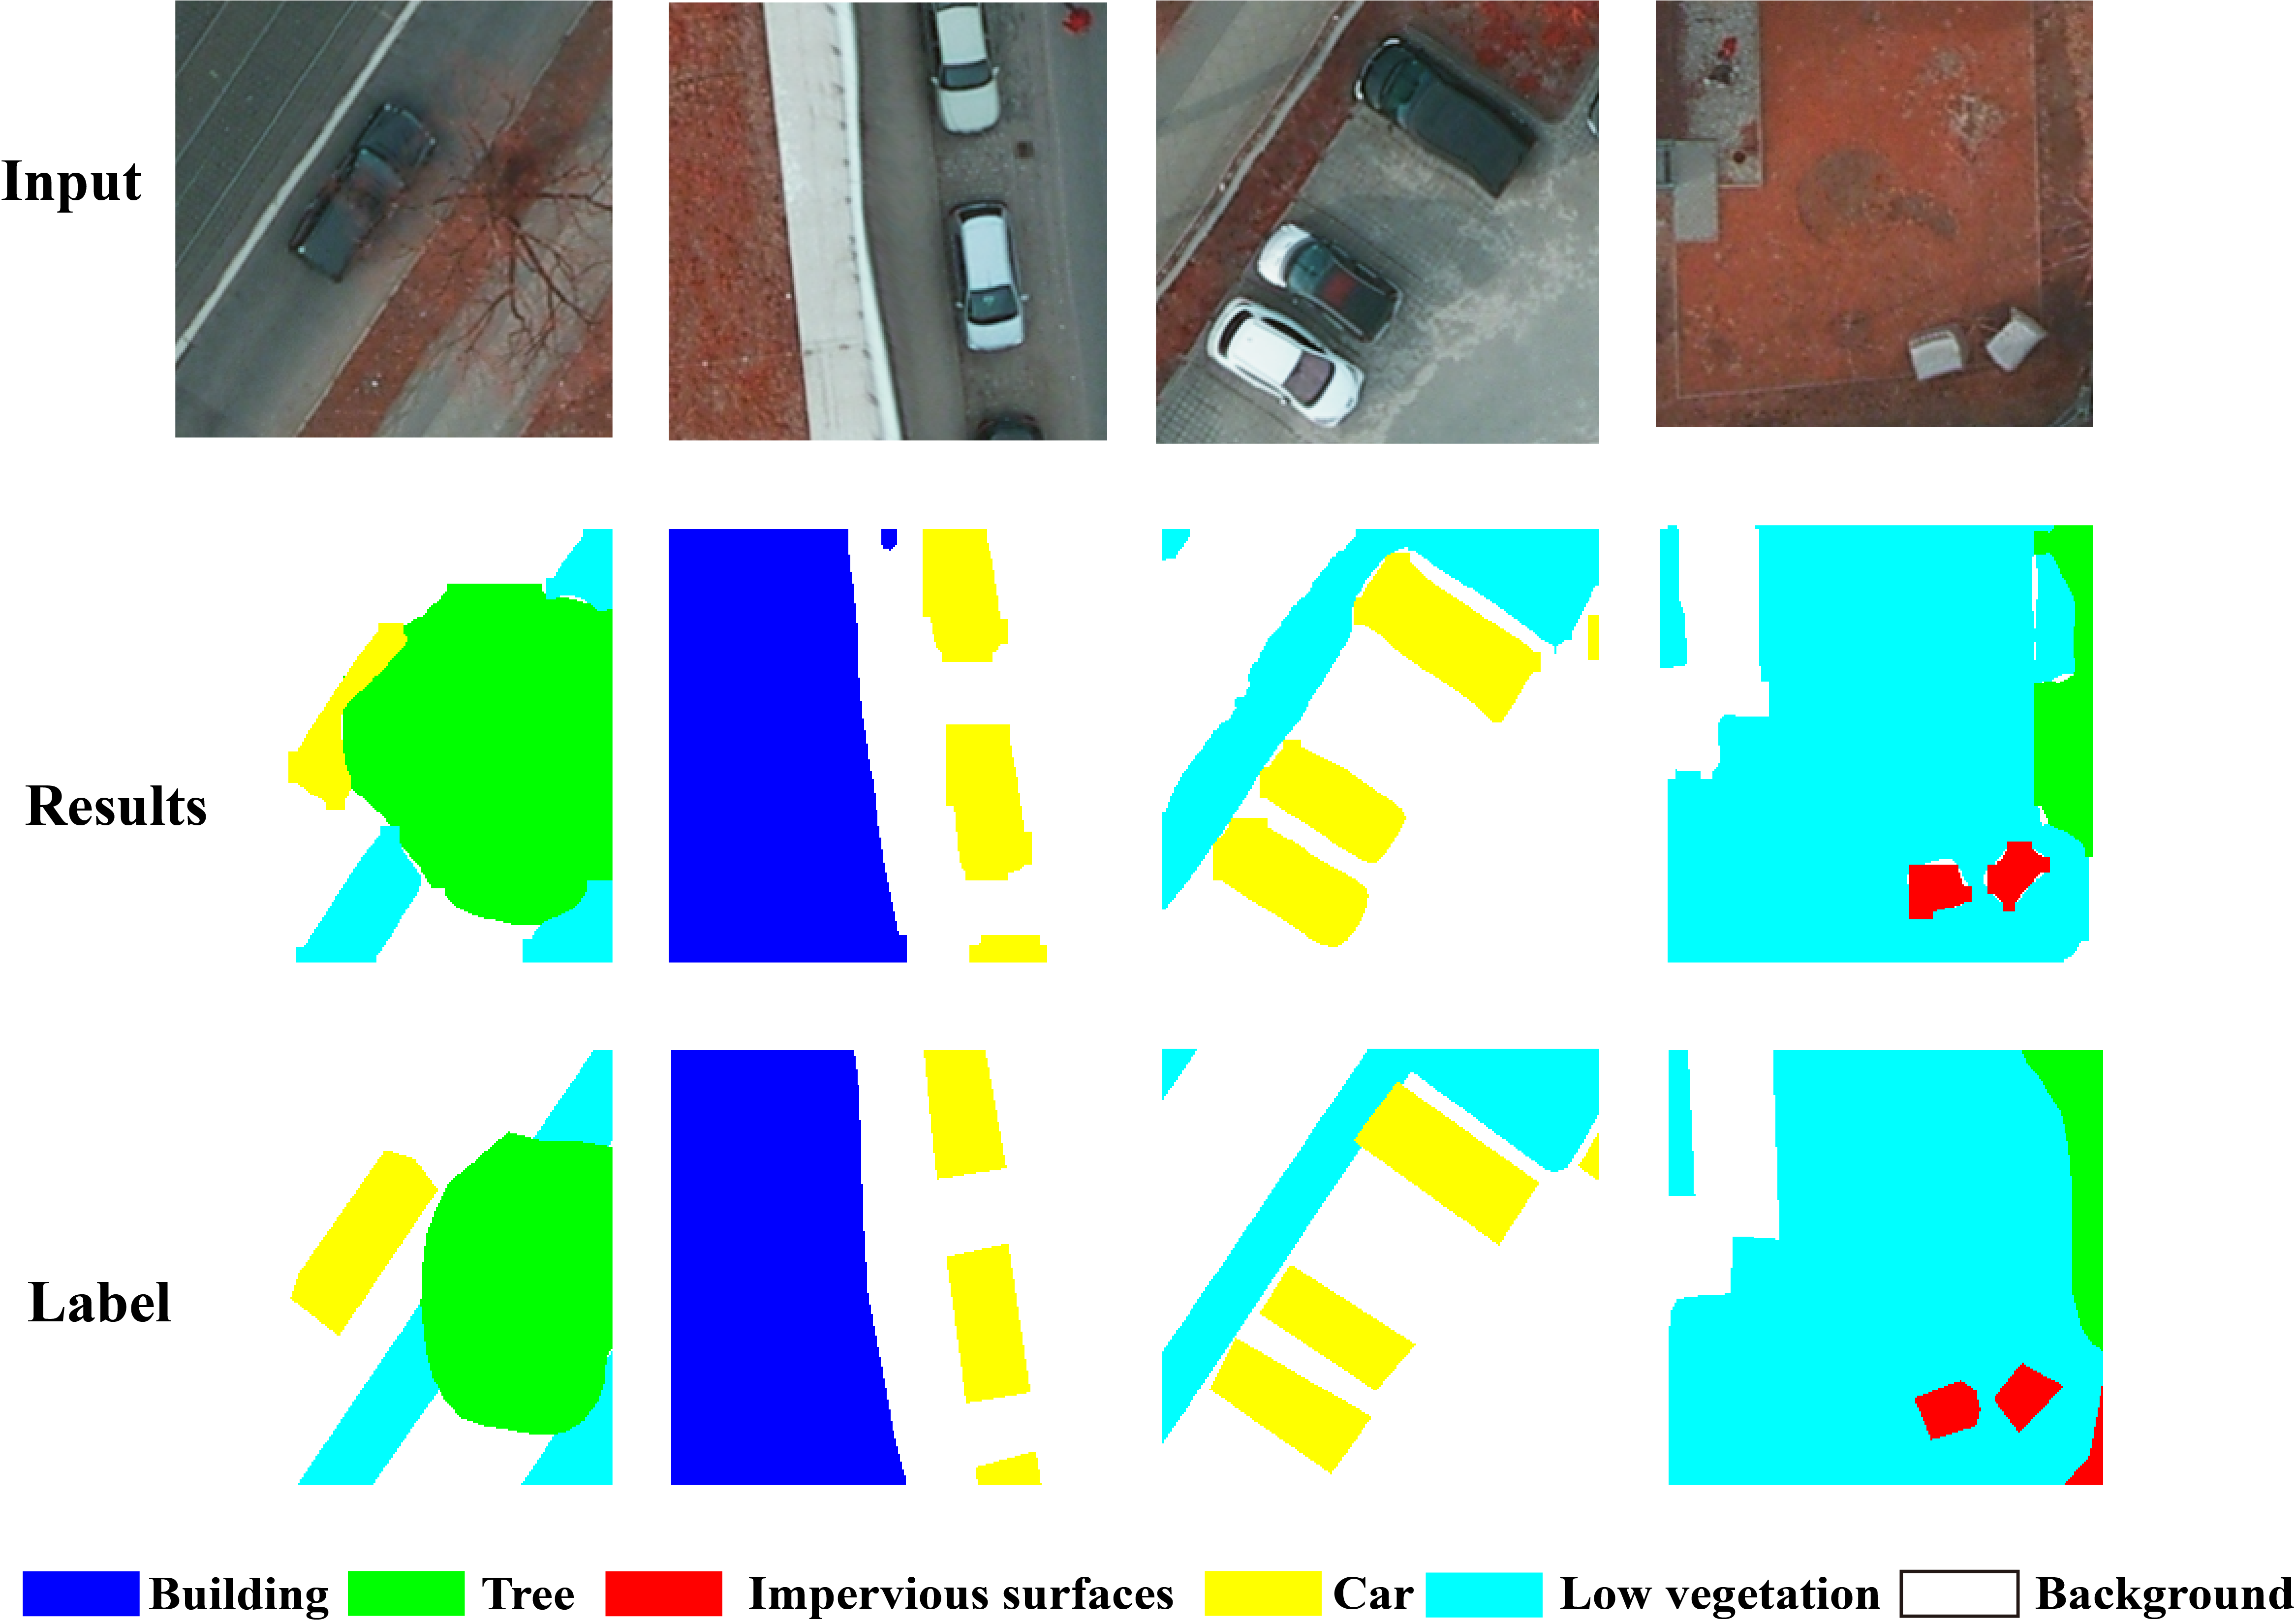
\includegraphics[width=8cm]{../image/8.png}
    \caption{Visualization of the segmentation results of the YOLO11x-Earth model on the Potsdam dataset.}
    \label{fig:segmentation-results}
\end{figure}
In conclusion, the pre-trained YOLO11-Earth backbone network demonstrated strong cross-task transfer learning 
capabilities, enabling the YOLO11-seg model to achieve rapid convergence and reasonable segmentation performance 
on the Potsdam dataset. This experiment confirmed the generalization ability of the YOLO11-Earth model across 
different tasks, further validating its potential as a lightweight open vocabulary detection model for remote 
sensing imagery.

\section{Cost-effectiveness and Interpretability}
\subsection{Cutting Down the Training Cost}
Currently, state-of-the-art (SOTA) models in the field of open vocabulary detection and open set detection, 
such as Grounding DINO and its 1.5 version, have adopted a training strategy similar to CLIP's text-image 
contrastive learning. Grounding DINO integrates a Transformer-based DINO detector with multi-modal pretraining, 
using composite datasets (detection, localization, classification, etc.) to align language and image content, 
thereby enabling the detection of arbitrary targets based on category names or descriptive expressions provided 
by humans. However, this approach inevitably incurs high training and inference costs. Grounding DINO requires 
64 Nvidia A100 GPUs to achieve a batch size of 64, and its 1.5 version, which aims to be more edge-friendly, 
still only achieves around 20 FPS on an A100 GPU without the acceleration of the TensorRT framework (compared 
to YOLO-Worldv2-L's inference speed of 37.4 FPS).

In contrast, the first real-time open vocabulary detection model, YOLO-World, and its v2 version almost 
entirely emulate Grounding DINO's training strategy. The key difference lies in the direct modification of 
the real-time object detection model YOLOv8, incorporating text information into the Rep-VL-PAN (corresponding 
to the neck of the original detector) and fusing image features with text information before performing text 
classification. This approach retains YOLOv8's real-time detection capabilities, with text feature classification 
activated only during training. Due to the simple model structure and fewer training datasets, YOLO-World reduces 
the training cost of open set target detection to 32 NVIDIA V100 GPUs, achieving a batch size of 512.

The best current remote sensing open vocabulary detection model, LAE-DINO, further reduces the cost of 
online multi-modal data fusion by constructing an offline large-scale rich-label detection dataset. This model 
moves the process of integrating multiple modalities online, as seen in Grounding DINO, to the data preparation 
phase, significantly reducing training costs. The authors of LAE-DINO explicitly state that their model is an 
improvement upon Grounding DINO. LAE-DINO's DVC module dynamically selects positive and negative vocabularies 
for each training batch, addressing the issue of large-scale vocabulary sets. The VisGT module enhances text 
features by introducing "scene features." These modifications enable LAE-DINO to be trained using only four 
A100 GPUs, with pretraining requiring approximately 180K steps and taking about 48 GPU hours. Of course, 
this does not account for the cost of generating the pretraining dataset using a pre-trained model.

In summary, the core idea of the representative models in the field of open vocabulary and open set detection 
is to interact language and image features during training as much as possible, ensuring that the features 
used for bounding box regression and label classification are as rich in semantic and image information as 
possible. This contrastive learning approach is the source of zero-shot transfer capabilities.
YOLO11-Earth explores a multi-modal method that does not involve contrastive learning training but simply 
integrates text features into the training process. Although our model does not achieve the zero-shot 
detection capability of models trained with contrastive learning on open sets, it factually endows 
the YOLO11 model, which should have no generalization capability, with zero-shot transfer capabilities 
on unseen datasets while retaining the fast fine-tuning capabilities of open set detectors (mainly compared 
to YOLO-Worldv2 and LAE-DINO). At the same time, the largest YOLO11x-Earth model only requires approximately 
60 hours of pretraining on a single NVIDIA RTX 4090 GPU, significantly reducing pretraining costs. The intuitive 
training cost comparison of the four models is shown in Table 8. The V100 GPU is assumed to have 32GB of 
memory by default, and the A100 GPU is assumed to have 80GB of memory by default.

\begin{table}[ht]
\centering
\caption{Comparison of training costs for different open vocabulary detection models.}
\begin{tabular}{lccc}
\toprule
\textbf{Model} & \textbf{GPU Model (Count)} & \textbf{Max Memory} & \textbf{Cost (per hour, USD, 5/13/2025)} \\
\midrule
Grounding DINO & NVIDIA A100 (64) & 5120GB & 59.35 \\
YOLO-World & NVIDIA V100 (32) & 1024GB & 8.35 \\
LAE-DINO & NVIDIA A100 (4) & 320GB & 3.71 \\
YOLO11-Earth & NVIDIA RTX4090 (1) & 24GB & 0.29 \\
\bottomrule
\end{tabular}
\end{table}

\subsection{Text Embedding as Bias}
To explain the principle behind YOLO11-Earth's ability to achieve open vocabulary detection using only the text 
content of labels, we first consider the encodable label mapping brought by the WorldDetect. This detection head 
that receives text features ensures that the classification of bounding boxes is within the given label range and 
can perform a certain "affine transformation" on the classification results based on new text feature inputs, 
namely translation and rotation. Relying on this detection head, YOLO11-Earth inherits the "prompt first, then 
detect" strategy of the YOLO-World architecture.

Secondly, in the forward process of YOLO11-Earth, all label text information is converted into text 
features by the CLIP text encoder and added to the input of each C2FAttn module and the WorldDetect detection 
head during forward propagation. This "addition" operation is essentially an affine transformation of the input 
feature vectors of each layer. Constructing a simple mapping can help us understand this process. Let the 
input data be denoted as a vector $x$, $x \in \mathbb{R}^n$, and the forward process of each layer in a 
multilayer perceptron can be represented as $f_i = W_i x + b_i$, where $i \in [1, m]$, $m$ is the number of 
layers in the neural network, and the activation function is denoted as $\sigma$. The output is $y$, and the 
mapping that the entire neural network attempts to fit is denoted as $g$. Assuming that all layers except the 
last one have activation functions, the output of a four-layer network can be written as:
\begin{equation}
y = g(x) = W_1 \cdot \sigma(W_2 \cdot \sigma(W_3 \cdot \sigma(W_4 x + b_4) + b_3) + b_2) + b_1
\end{equation}
In essence, a deep learning model is a complex non-linear mapping composed of a series of linearly combined 
parameter layers, and the parallel operations within each layer can be understood as operations on the blocks 
of the matrix $Wx+b$. Assuming the first layer represents the output of the model's backbone network (without 
text features $t$), then the operation of adding text features in the neck and detection head parts of 
YOLO11-Earth can rewrite the mapping as:
\begin{equation}
y = g(x) = W_1 \cdot \sigma(W_2 \cdot \sigma(W_3 \cdot \sigma(W_4 x + b_4 + t) + b_3 + t) + b_2 + t) + b_1
\end{equation}
Intuitively, the text feature $t$ added at each step causes a fixed offset in the output of the previous layer. 
We can visualize the distributions of $y$ obtained before and after adding $t$ to test the above inference.
\begin{figure}[htbp]
    \centering
    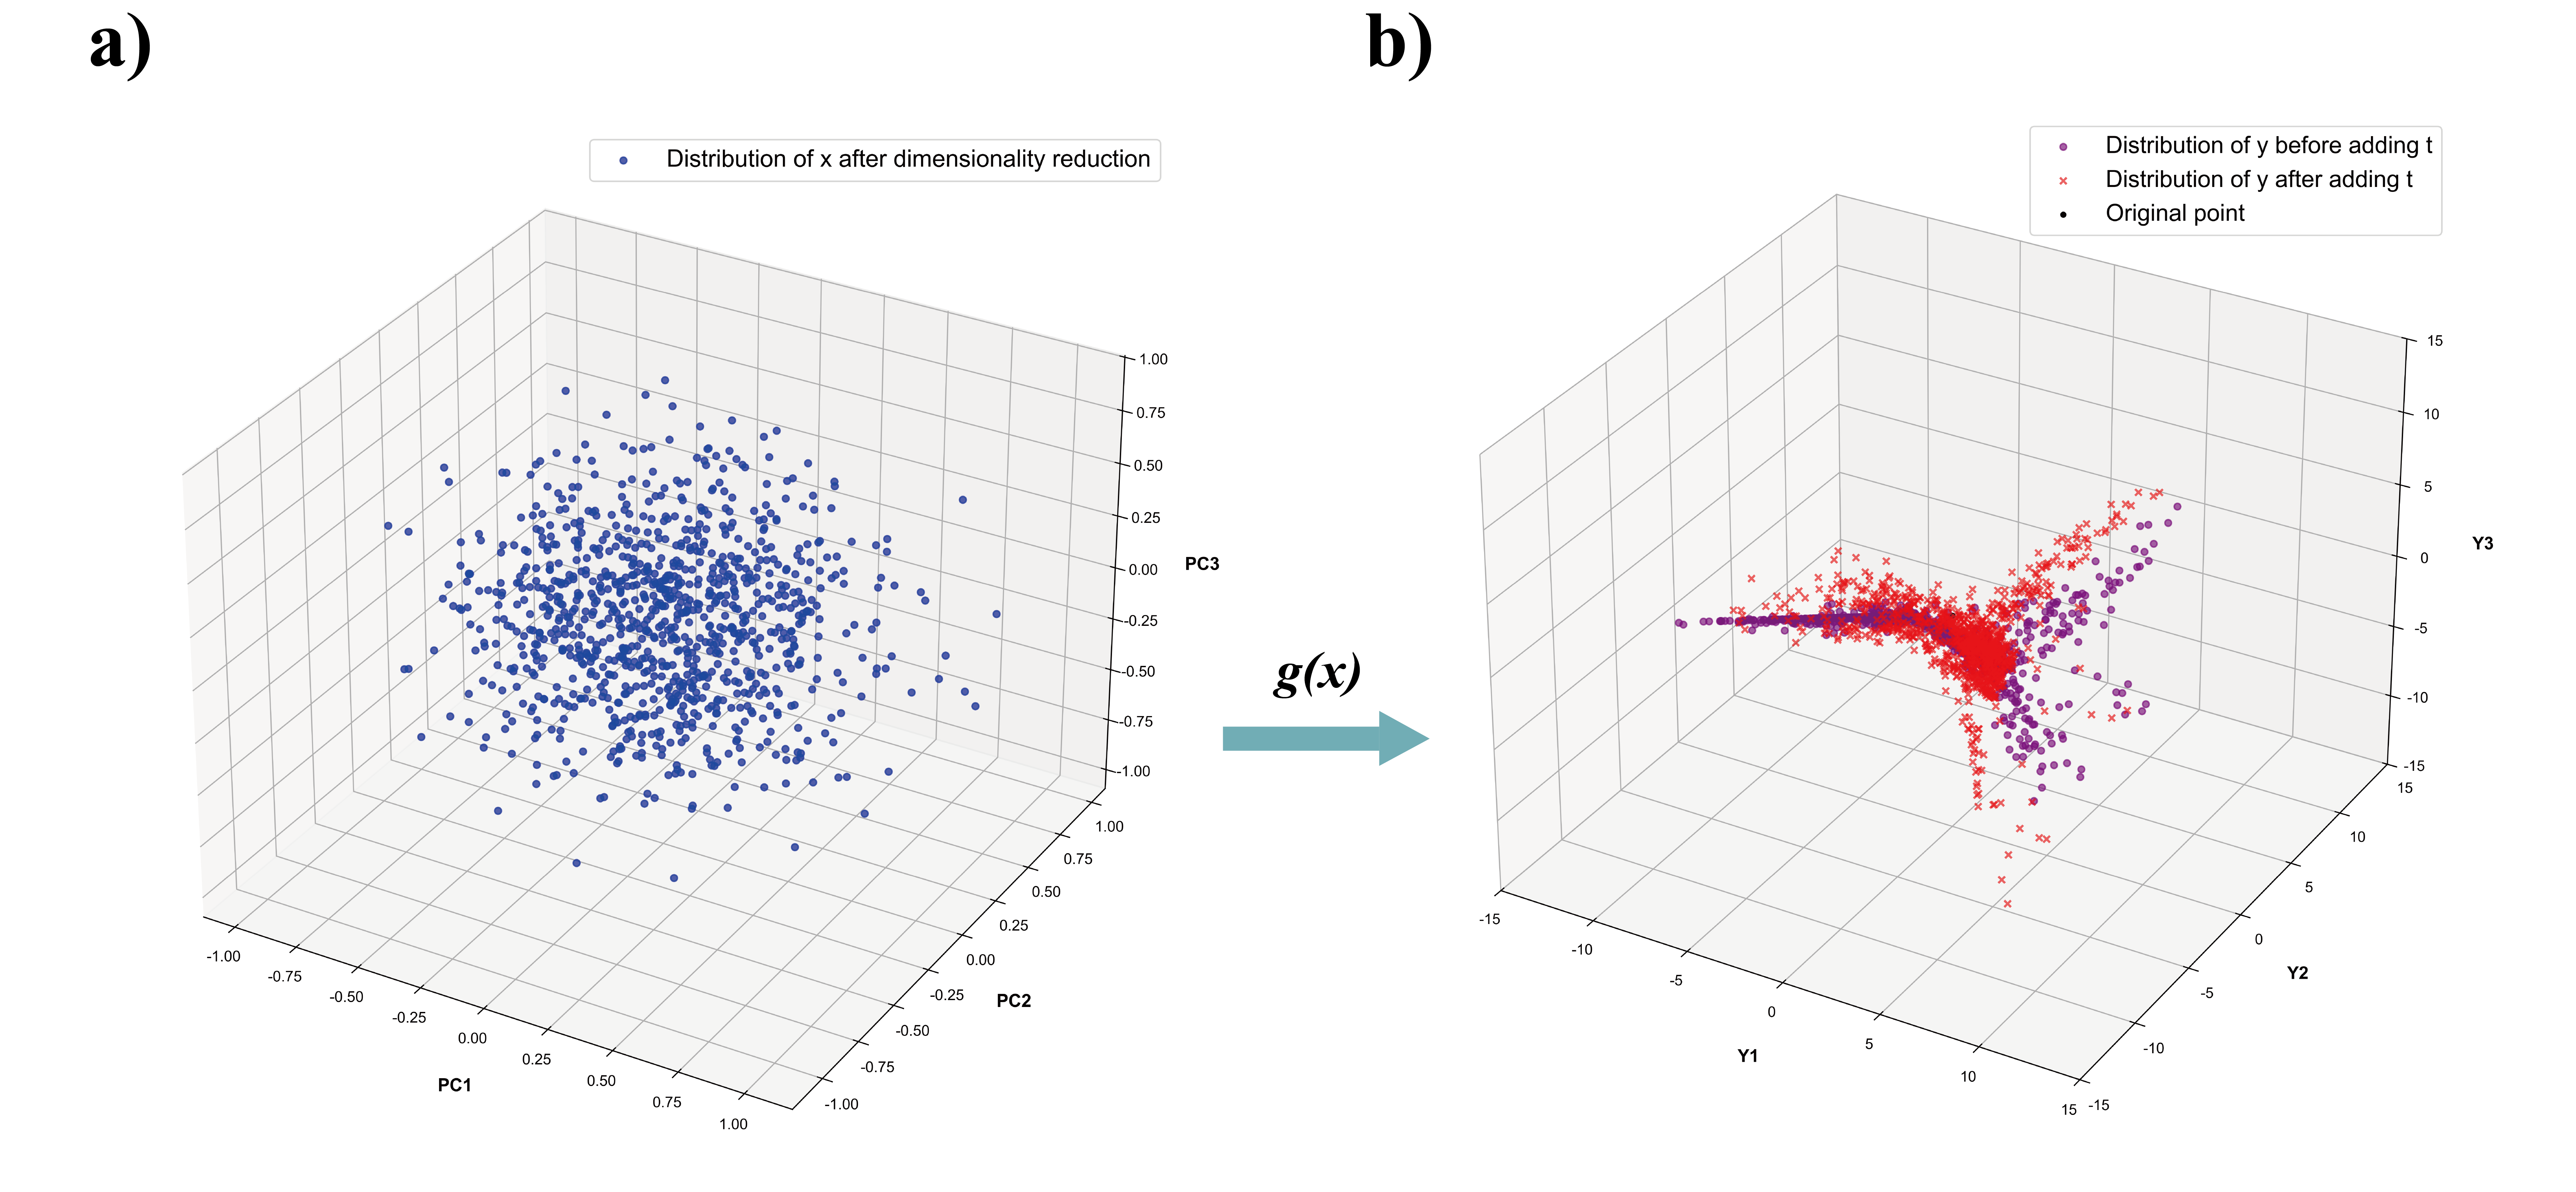
\includegraphics[width=12cm]{../image/9.png}
    \caption{Visualization of the distribution shift caused by text features. (a) Original 6D input data 
    reduced to 3D using PCA. (b) Output distribution before (purple) and after (red) adding text features, 
    showing clear separation in the distribution spaces.}
    \label{fig:distribution-shift}
\end{figure}
Figure 9 shows the change in the distribution of $y$ before and after adding the constant feature $t$. 
The 6-dimensional input variable $x$ is reduced to 3 dimensions using PCA for visualization purposes. 
A set of 1000 points randomly sampled from a 6-dimensional Gaussian distribution, with each dimension 
normalized to $[-1,1]$, is used as input. A random 6-dimensional vector $t$ is generated to mimic the text 
feature vector, and the distribution of $y$ is obtained using the aforementioned formula. The weights and 
biases of the first three layers are set to ensure that the dimension of $x$ remains unchanged (6 dimensions), 
and ReLU is used as the activation function after the third layer.

As can be observed, the distribution of y obtained using only image features (purple points in Figure 9b) 
exhibits a discernible difference from the distribution of y after incorporating the text feature t (red points 
in Figure 9b). This discrepancy is evident in both the mean and variance of the distributions. Consequently, 
when these distinct distributions are subjected to classification via a fully connected layer, the resulting 
classifications will naturally diverge.

This visualization elucidates why YOLO11-Earth, despite the absence of contrastive learning during training 
to align text and image features, still acquires a rudimentary capability for open-set detection. This capability 
stems from the affine transformation (vector addition) imposed on the intermediate output of each layer by the 
text features. This operation sacrifices the fitting of the original image feature distribution to some extent 
but enhances the alignment with the text feature distribution. The reason YOLO11-Earth's zero-shot transfer 
capability falls short of models trained with contrastive learning alignment is that the text features in 
YOLO11-Earth remain constant throughout the forward pass and are merely added to the image features. This offset 
is insufficiently strong to achieve robust alignment.

In conclusion, YOLO11-Earth's open vocabulary detection capability, while not on par with models trained 
using contrastive learning, is nonetheless a significant achievement given its minimal training cost. This 
capability is rooted in the affine transformation induced by the text features, which, despite its simplicity, 
enables the model to generalize to unseen datasets. This finding underscores the potential for lightweight models 
to achieve open vocabulary detection with significantly reduced computational resources, paving the way for 
more accessible and efficient remote sensing applications.

\subsection{ Limitations}
Despite the significant improvements offered by YOLO11-Earth in the context of open vocabulary detection for 
remote sensing imagery, several limitations persist. One notable limitation is its terrible zero-shot transfer 
capability when compared to models trained with contrastive learning. This is primarily attributed to 
YOLO11-Earth's reliance on closed-set training data, which inherently restricts its ability to generalize 
across diverse datasets. The model's performance is further constrained by the absence of updated text features 
and the lack of specialized loss functions designed to optimize text feature learning. These factors collectively 
result in YOLO11-Earth underperforming in zero-shot scenarios where models are expected to recognize novel 
categories without additional training.

Moreover, the model encounters challenges when deployed across different remote sensing datasets due to the 
inherent variability in sensor types and imaging conditions. This is exacerbated by the specific characteristics 
of remote sensing data, such as high dimensionality and complex background noise, which can lead to suboptimal 
performance if not adequately addressed. The model's architecture, while efficient, may not fully capture the 
intricate patterns and nuances present in remote sensing imagery, thereby limiting its detection accuracy and 
reliability.

\section{Conclusion}
This technical report has introduced YOLO11-Earth, a lightweight open vocabulary detection model designed for 
remote sensing imagery. Built upon the foundations of YOLOv11 and YOLOv8-Worldv2, YOLO11-Earth leverages model 
pruning and innovative VL-PAN design to achieve real-time open vocabulary detection capabilities on conventional 
datasets and consumer-grade GPUs. Extensive experiments across various benchmarks have demonstrated 
YOLO11-Earth's superior performance in terms of detection accuracy, computational efficiency, and 
cross-dataset generalization. These findings underscore the model's potential to serve as a versatile 
and cost-effective solution for a wide array of remote sensing applications.

However, the report also highlights several avenues for future improvement. Enhancing YOLO11-Earth's zero-shot 
transfer learning capabilities represents a key area for development. This could be achieved by refining 
the model's text feature encoding mechanisms and incorporating more sophisticated cross-modal alignment 
techniques. Additionally, expanding the diversity and scale of training datasets would better equip the model 
to handle the complexities and variabilities of real-world remote sensing data. Further exploration into 
advanced model architectures and training strategies, such as incorporating attention mechanisms and employing 
more efficient feature extraction methods, could also significantly boost YOLO11-Earth's performance. The 
ultimate goal is to create a more powerful and adaptable open vocabulary detection model that can reliably 
and accurately detect objects across various remote sensing datasets and scenarios.

In summary, while YOLO11-Earth has made significant strides in the field of lightweight remote sensing open 
vocabulary detection, ongoing research and development efforts are necessary to overcome its limitations and 
unlock its full potential. By addressing the identified challenges, future open-vocabulary detectors can be 
expected to deliver even more impressive results and further advance the capabilities of remote sensing object 
detection technologies, with low cost and high performance.

\bibliography{refs.bib}%refs.bib
\end{document}